\documentclass[review]{elsarticle}
%\documentclass[3p,times,twocolumn,authoryear]{elsarticle}

\usepackage{amssymb}
\usepackage{multirow}
\usepackage{booktabs}
\usepackage[colorlinks,urlcolor=blue]{hyperref}
\usepackage{subfig}
\usepackage{scalefnt}
\usepackage[brazilian]{babel}
\usepackage[utf8]{inputenc}
\usepackage[T1]{fontenc}
\usepackage{units}
\usepackage{url}
\usepackage{amsbsy}
\usepackage{amstext}
\usepackage{graphicx}
\usepackage{rotating}
\usepackage{xcolor}
\usepackage{float}
\usepackage[section]{placeins}
\usepackage{verbatim}
\usepackage{apalike}
\restylefloat{figure}
\restylefloat{table}

% Inserted by pgirardi
\usepackage{amsmath}
\usepackage[normalem]{ulem}
% ponytail: \texttt só — \seqsplit quebra com \_ / babel brazilian
\newcommand{\code}[1]{\texttt{#1}}

% \newcommand{\sugestao}[1]{\textcolor{blue!100!black}{\textbf{#1}}}

\newcommand{\sugestao}[2]{%
	\textcolor{red}{\sout{\textbf{#1}}}%
	\textcolor{blue!100!black}{\textbf{#2}}%
}

%%%%%%%%%%%%%%%

\makeatletter

\journal{Expert Systems with Applications}

\@ifundefined{showcaptionsetup}{}{%
	\PassOptionsToPackage{caption=false}{subfig}}
\usepackage{pdflscape}
\@ifundefined{showcaptionsetup}{}{%
	\PassOptionsToPackage{caption=false}{subfig}}
\makeatother


\begin{document}
	\begin{frontmatter}
		
		\title{Representação longitudinal hipocampal para sMCI versus pMCI:
			alteração temporal, coortes multi-janela e fusão multimodal}
		
		\author[ufscar]{Paulo Matheus da Costa Girardi}
		\ead{paulogirardi@estudante.ufscar.br}
		
		\author[ufscar]{Ricardo José Ferrari\corref{cor1}}
		\ead{rferrari@ufscar.br}
		
		\cortext[cor1]{Corresponding author}
		
		\address[ufscar]{Department of Computing, Federal University of São Carlos, Rod.\ Washington Luis, Km 235, 13565-905, São Carlos, SP, Brazil}
		
		\author[]{for the Alzheimer's Disease Neuroimaging Initiative\corref{adni}}
		\cortext[adni]{Data used in preparation of this article were obtained from the Alzheimer's Disease Neuroimaging Initiative (ADNI) database (\url{adni.loni.usc.edu}). Investigators within ADNI contributed to the design and implementation of ADNI and/or provided data but did not participate in analysis or writing of this report. A complete listing of ADNI investigators is available at \url{http://adni.loni.usc.edu/wp-content/uploads/how_to_apply/ADNI_Acknowledgement_List.pdf}.}
		
		\begin{abstract}
			Distinguir sMCI de pMCI no hipocampo com RM T1 isolada é difícil: o sinal é subtil e a literatura mistura janelas, ROIs e validação.
			Neste estudo (ADNI-1/2/GO) pergunta-se se a representação \code{t1\_deltas} --- atributos de $t_0$ mais diferenças de nível $T_b-T_a$ entre três visitas --- agrega informação relativamente a \code{t1\_only}.
			O contraste corre em quatro famílias (volume, forma, textura GLCM, deslocamento) e em quatro coortes (janelas 36/48\,meses $\times$ intervalos nominais 6/12\,meses, tolerância $\pm 2$).
			A concatenação \code{wide} é só âncora metodológica: níveis em três visitas não medem mudança.
			Protocolo fixo: SVM, pool L1 por frequência (\code{l1\_stable}, $\tau=70\%$), sem ComBat, CV aninhada no paciente ($5\times 10$); métrica primária AUC de Mann--Whitney sobre a média das probabilidades OOF por sujeito.
			A textura tem $\Delta\mathrm{AUC}>0$ nas quatro células (máximo $+0.058$ em \code{48m\_12m}, $n=120$); a forma é um teto estático no $t_0$; o volume é misto; o deslocamento é fraco.
			Nenhum $\Delta$ unimodal retém $q<0.05$ após FDR de Benjamini--Hochberg.
			A fusão tardia forma@$t_0$ $\cup$ textura-$\Delta$ atinge $0.801\pm0.040$ em \code{48m\_12m}, acima da forma no baseline ($0.761\pm0.043$), mas os escores clínicos de $t_0$ (sexo, idade, MMSE, ADAS, FAQ) chegam a $0.812$ e o ganho fusão clínica$+$imagem versus clínico não é significativo.
			A RM hipocampal entra como adjunto estrutural, não como primeira linha.
		\end{abstract}
		
		\begin{keyword}
			Longitudinal MRI \sep hippocampus \sep Mild Cognitive Impairment \sep Radiomics \sep Machine Learning \sep Nested cross-validation \sep Late fusion
		\end{keyword}
		
	\end{frontmatter}
	
	% =============================================================================
	\section{Introdução}
	\label{sec:introducao}
	
	A doença de Alzheimer (AD) e o comprometimento cognitivo leve (MCI) situam-se num contínuo de declínio~\cite{petersen-1999}.
	Identificar quais indivíduos com MCI permanecerão estáveis (sMCI) e quais progredirão para demência (pMCI) interessa a enriquecimento de ensaios, aconselhamento e planeamento de intervenção~\cite{petersen-2009}.
	A RM estrutural T1-ponderada permanece central nesse problema, e a atrofia hipocampal é um dos marcadores macroscópicos mais consolidados~\cite{scheltens-1992}.
	Na fronteira sMCI/pMCI, contudo, a discriminação a partir de uma única região é intrínsecamente difícil: as diferenças de grupo são subtis, a dinâmica de conversão é heterogénea e a alteração estrutural sobrepõe-se ao envelhecimento.
	
	Uma literatura ampla recorreu a representações mais ricas --- morfometria de cérebro inteiro, fusão com escores cognitivos, radiómica e aprendizagem profunda longitudinal~\cite{moradi-2015,ye-2012,zhang-2019,lin-2020,aghajanian-2025}.
	As AUC reportadas podem ser altas, mas a comparabilidade é limitada.
	Coortes, definições de desfecho (p.ex.\ ncMCI/cMCI, conversão MCI$\to$AD num horizonte fixo), escala espacial (cérebro inteiro versus ROI), entrada temporal (só baseline versus visitas repetidas) e desenho de validação diferem.
	Além disso, muitos pipelines aplicam harmonização, selecção de atributos, ajuste de hiperparâmetros ou limiar de decisão com informação do conjunto completo ou das partições de teste, e nem todos impõem divisão estrita no nível do paciente.
	Sob essas condições, AUC otimistas são difíceis de interpretar e podem não reflectir o desempenho atingível com validação no paciente e ajuste fold-wise.
	
	Este estudo avalia um fluxo auditável de extração de atributos hipocampais e classificação prognóstica na ADNI (ADNI-1/2/GO).
	O hipocampo foi escolhido de propósito como marcador canónico de atrofia e como banco de teste longitudinal, não como cobertura prognóstica de cérebro inteiro.
	A cadeia documentada cobre pré-processamento T1, controlo de qualidade, parcelamento, registro a templates e extração de atributos volumétricos, morfométricos, texturais e de campo de deslocamento no hipocampo.
	O desempenho avalia-se com validação cruzada aninhada no paciente; o filtro de frequência $\ell_1$ por bootstrap restringe-se ao treino de cada dobra externa, e a harmonização ComBat fold-wise entra só como análise de sensibilidade.
	A novidade está na arquitectura de avaliação, não num classificador novo: elegibilidade temporal, apuração do desfecho, divisão por paciente, operações ajustadas só no treino, selecção específica da representação, agregação de probabilidades e comparações com correcção de multiplicidade formam uma cadeia auditável.
	Esse desenho permite comparar, no mesmo estimando, \code{t1\_deltas} versus \code{t1\_only}, a âncora \code{wide}, preditores clínicos e fusões, e identificar o que permanece informativo depois dos controlos de vazamento e do FDR.
	
	\paragraph{Pergunta.}
	No hipocampo, para sMCI versus pMCI, há alteração temporal útil além do que a imagem de baseline já mostra?
	Quantifica-se $\Delta\mathrm{AUC}=\mathrm{AUC}(\code{t1\_deltas})-\mathrm{AUC}(\code{t1\_only})$ em quatro famílias de atributos e nas quatro células do fatorial janela clínica $\times$ intervalo entre imagens.
	
	Contribuições para avaliação reprodutível em neuroimagem longitudinal:
	\begin{itemize}
		\item protocolo que separa visitas preditoras em estágio MCI da apuração do desfecho e documenta a fronteira de ajuste de cada operação dependente da amostra sob validação aninhada no paciente;
		\item matriz controlada em quatro famílias hipocampais, representações $t_0$ versus $t_0$+deltas, quatro coortes, fusão tardia versus precoce, preditores clínicos e ComBat, sob o mesmo estimando de AUC no paciente (SVM; RF, elastic-net e MLP só em sensibilidade);
		\item inferência além do ponto: permutação de rótulos no paciente, intervalos bootstrap pareados do $\Delta$AUC e FDR de Benjamini--Hochberg;
		\item evidência de apoio à decisão: variáveis clínicas baratas permanecem o sinal de primeira linha nesta coorte; a RM hipocampal é adjunto estrutural cuja contribuição incremental deve ser demonstrada, não presumida.
	\end{itemize}
	
	O desfecho primário é a classificação binária sMCI versus pMCI.
	O restante do artigo organiza-se assim: a Secção~\ref{sec:metodos} descreve coorte, extração de atributos e validação; a Secção~\ref{sec:resultados} reporta os resultados prognósticos e comparativos; a Secção~\ref{sec:discussao} discute achados e limitações; a Secção~\ref{sec:conclusoes} conclui.
	
	
\subsection{Trabalhos relacionados}
\label{subsec:relacionados}

A previsão automática de estabilidade ou conversão do MCI foi estudada com conjuntos de atributos, esquemas de validação e janelas de desfecho muito distintos.
Na investigação prognóstica baseada na ADNI, MCI estável e progressivo aparecem também como ncMCI/cMCI ou MCInc/MCIc, clinicamente análogos a sMCI e pMCI.
O desempenho depende, portanto, não só do classificador, mas de os preditores serem clínicos, estruturais, multimodais, regionais ou de cérebro inteiro, e de a informação temporal limitar-se ao baseline ou cobrir várias visitas de seguimento.

Vários estudos mostram que o acompanhamento cognitivo denso pode ser informativo mesmo sem RM.
\citet{bucholc-2023} propuseram um ensemble híbrido no National Alzheimer's Coordinating Center (NACC) para prever conversão MCI$\to$demência a partir de trajectórias cognitivas e funcionais.
A acurácia de classificação atingiu $85{,}0$--$87{,}5\%$, mas a AUC do ensemble no teste retido ficou perto de $0.60$, ao passo que florestas aleatórias chegaram a AUC até $0.76$ quando havia quatro visitas.
\citet{grassi-2019} previram conversão a 3 anos na ADNI só com variáveis sociodemográficas e neuropsicológicas e reportaram AUROC $0.88$ (IC bootstrap 95\%: $0.85$--$0.91$), com sensibilidade $77{,}7\%$ e especificidade $79{,}9\%$ no ponto de melhor acurácia balanceada.
Esses resultados indicam que o rastreio clínico carrega sinal prognóstico substancial e constitui um comparador forte para modelos só de imagem.

Estudos de RM estrutural recorrem frequentemente a representações de cérebro inteiro de alta dimensão ou a fusão com escores cognitivos.
\citet{moradi-2015} aplicaram \emph{low-density separation} a T1 de baseline da ADNI para previsão precoce de conversão em MCI, com AUC $0.766$ em morfometria voxel-a-voxel isolada e AUC $0.902$ ao combinar RM com um agregado cognitivo de baseline.
\citet{ye-2012} usaram selecção estável esparsa (Biosignature-15) para prever conversão MCI$\to$AD em quatro anos, com AUC $0.859$ em validação leave-one-out (LOOCV) na ADNI de baseline.
\citet{casanova-2013} combinaram atributos de RM em larga escala, baseados em tecido, com informação cognitiva num quadro de avaliação de risco por aprendizagem automática na ADNI.
Tais estudos mostram que AUC altas surgem sobretudo com desenhos de cérebro inteiro ou multimodais, e com definições de desfecho que podem diferir da discriminação sMCI/pMCI em horizonte curto e regras estritas.

Quando o âmbito espacial se reduz a uma única ROI, o desempenho em geral cai.
\citet{cuingnet-2011} compararam dez métodos de classificação na ADNI e reportaram que a discriminação conversor versus não conversor, inclusive com atributos de volume hipocampal, não excedeu o acaso de forma significativa.
\citet{guo-2017a} estudaram espessura cortical relacionada com conversão para sMCI versus cMCI, com acurácia $98{,}84\%$ e sensibilidade/especificidade $97{,}5/100$ em LOOCV, mas sem reportar AUC.
Esses achados são coerentes com a ideia de que restringir a análise a uma região focal --- hipocampo ou córtex --- produz desempenho prognóstico mais conservador do que modelos voxel de cérebro inteiro.

Trabalho mais recente incorpora RM temporal via aprendizagem de dicionários, redes profundas ou radiómica.
\citet{zhang-2019} analisaram RM estrutural longitudinal para classificação AD/MCI, \citet{lin-2020} usaram aprendizagem de dicionários longitudinal para prever progressão MCI$\to$AD, e \citet{aghajanian-2025} combinaram aprendizagem profunda com radiómica de RM estrutural longitudinal para previsão de progressão.
Essas abordagens mostram interesse crescente em modelação temporal, mas diferem em definição de coorte, controlo de vazamento e comparação com baselines clínicos.

Neste contexto, o presente trabalho não visa reproduzir o estado da arte de cérebro inteiro multimodal.
Visa especificar e estressar um pipeline prognóstico focado no hipocampo na ADNI, com configuração primária pré-especificada (SVM, filtro de frequência L1 por bootstrap, sem ComBat, AUC no paciente) e ablações sistemáticas: quatro famílias de atributos, \code{t1\_deltas} versus \code{t1\_only} (com \code{wide} só como âncora metodológica), quatro células janela$\times$intervalo, preditores clínicos e fusão multimodal.
A contribuição original é o protocolo de avaliação coordenado: todas as representações candidatas correm sob elegibilidade temporal explícita, validação aninhada no paciente, ajuste fold-wise, o mesmo estimando OOF e comparações com correcção de multiplicidade.
Ablações negativas e positivas tornam-se evidência de desenho para futuros sistemas de apoio à decisão, em vez de tratar a maior AUC observada como único resultado.
Sob esse protocolo, a forma no $t_0$ atinge AUC paciente $\approx 0.76$ em \code{48m\_12m}; a fusão tardia âncora chega a $\approx 0.80$; os escores clínicos de $t_0$ permanecem competitivos ($\approx 0.81$).
Nenhum $\Delta$AUC unimodal sobrevive ao FDR.
A Tabela~\ref{tab:literature_comparison} resume literatura representativa ao lado destes resultados, sob definições de tarefa heterogéneas mas clinicamente análogas.
	
	% =============================================================================
	\section{Material e métodos}
	\label{sec:metodos}
	
	\subsection{Definição da coorte}
	\label{sec:populacao}
	
	
	Os dados utilizados neste estudo foram obtidos da base de dados da Alzheimer's Disease Neuroimaging Initiative (ADNI)~\cite{petersen-2009,jr-2008}.
	A ADNI foi lançada em 2003 como parceria público--privada para avaliar marcadores clínicos, genéticos, bioquímicos e de neuroimagem longitudinais da doença de Alzheimer (AD).
	Este estudo utilizou RM estrutural T1-ponderada adquirida com sequências tridimensionais Magnetization-Prepared Rapid Gradient-Echo (MP-RAGE) das fases ADNI-1, ADNI-2 e ADNI-GO, coletadas em centros nos Estados Unidos e no Canadá em scanners de 1.5~T e 3~T da GE Healthcare, Philips Medical Systems e Siemens Medical Solutions.
	
	A coleção ADNI inicial compreendia 15{,}016 imagens de 1{,}495 participantes.
	Duas imagens de um participante com designação de sexo inválida foram excluídas, restando 15{,}014 imagens de 1{,}494 participantes.
	
	O controle de qualidade foi aplicado a esse conjunto completo de volumes T1, ainda sem rótulos diagnósticos e antes da construção das coortes.
	Métricas de qualidade de imagem (IQMs) de referência livre foram calculadas com \code{MRQy}~\citep{sadri-2020}.
	Candidatos a outliers foram rastreados com as métricas \code{VRX}, \code{COL}, \code{NUM}, \code{CPP}, \code{PSNR}, \code{SNR7}, \code{CNR}, \code{CVP}, \code{CJV}, \code{EFC} e \code{FBER}, escolhidas pela relevância a recorte de FOV, geometria de aquisição, ruído e degradação relacionada a movimento ou artefato.
	Para cada métrica, outliers foram definidos pelas cercas de Tukey~\citep{tukey-1977},
	\begin{equation}
		\left[Q_1 - \alpha\,\mathrm{IQR},\, Q_3 + \alpha\,\mathrm{IQR}\right],
		\qquad \mathrm{IQR} = Q_3 - Q_1,
		\label{eq:tukey}
	\end{equation}
	com $\alpha = 1.5$ e direcionalidade específica da métrica (valores baixos indesejáveis, altos indesejáveis, ou bilateral).
	Cada volume recebeu uma pontuação de não conformidade igual ao número de IQMs sinalizadas; volumes com pontuação $\geq 3$ entraram em uma lista curta ($69/15{,}014$; $0.46\%$).
	Os quartis e os limites de IQR foram estimados uma única vez a partir desse conjunto de 15{,}014 volumes, sem rótulos diagnósticos, antes da construção das coortes e da validação cruzada; não foram recalculados nas partições externas.
	Esse rastreio ao nível do conjunto de dados foi, portanto, distinto da modelagem ajustada por partição.
	Todos os casos da lista curta foram inspecionados visualmente no ITK-SNAP~\citep{yushkevich-2006} (v4.2.0).
	A inspeção confirmou 12 identificadores de aquisição para exclusão por FOV incompleto, aquisições danificadas ou faixas de ruído estruturado.
	
	Em seguida procedeu-se à construção da coorte clínica.
	Na ADNI, o diagnóstico associado à primeira visita (baseline) não acompanha necessariamente a progressão longitudinal; por isso, cada exame de RM foi alinhado ao diagnóstico clínico e às escalas cognitivas/funcionais (ADAS, CDR, MMSE, FAQ) por correspondência temporal, exigindo distância absoluta $\leq 3$ meses ($\pm 90$ dias) entre a data de aquisição e a data da avaliação clínica, de modo que o rótulo corresponda o mais possível ao momento da imagem.
	Assim, imagens do mesmo paciente podem receber rótulos clínicos distintos ao longo do tempo.
	Antes do pareamento imagem--diagnóstico, os registros diagnósticos longitudinais foram filtrados: removeram-se demências diferentes da doença de Alzheimer, diagnósticos ou datas em falta, e reversões clinicamente implausíveis nas fases contínuas da AD --- MCI$\rightarrow$CN ou AD$\rightarrow$MCI/CN.
	Esse rastreio identificou 40 participantes com reversão a partir de AD e, após a sua remoção, mais 128 com reversão MCI$\rightarrow$CN, totalizando 168 participantes únicos excluídos; destes, 112 estavam representados na coleção de imagem e correspondiam a 1{,}325 imagens.
	O pareamento RM--diagnóstico na janela de $\pm 90$ dias excluiu mais 666 imagens, e a exigência de escores clínicos completos excluiu outras 92, resultando em 12{,}931 imagens rotuladas de 1{,}304 participantes.
	Dos 12 identificadores rejeitados pelo controle visual de qualidade, 10 ainda estavam presentes após o pareamento clínico e foram removidos nesta etapa; os outros dois já tinham sido eliminados pelos filtros diagnósticos precedentes.
	A tabela após o controle de qualidade continha, portanto, 12{,}921 imagens.
	A remoção de 3{,}757 aquisições cuja descrição ADNI as identificava como repetições (\emph{repeats}) reduziu o conjunto a 9{,}164 candidatas longitudinais utilizáveis.
	Esse pool de 9{,}164 imagens é o ponto de partida para a formação dos conjuntos longitudinais descritos a seguir; ainda não coincide com a coorte final de análise (Tabela~\ref{tab:adni_study}), que resulta da exigência de exatamente três imagens por paciente sob as regras de janela clínica e intervalo entre aquisições.
	
	
	\subsubsection{Formação dos conjuntos}
	\label{subsec:formacao}
	
	A formação de cada conjunto longitudinal segue duas etapas em sequência, para que o rótulo clínico não dependa de qual imagem acabou sendo escolhida como preditora.
	
	\paragraph{Etapa 1 --- rótulo clínico.}
	Para cada paciente, ordenam-se todas as suas RM pela data de aquisição.
	A data da primeira RM define o instante de referência $t_0$ (baseline).
	Sobre esse instante fixa-se uma \textbf{janela de observação clínica} de 36 ou 48 meses, com término em $t_{\mathrm{end}} = t_0 +$\,janela.
	Olhando toda a trajetória diagnóstica do paciente (não apenas três imagens), decide-se se ele é CN, sMCI, pMCI, AD, ou se deve ser excluído.
	Só depois dessa decisão passa-se à escolha das imagens que alimentarão o modelo.
	
	\paragraph{Etapa 2 --- três imagens preditoras.}
	Cada paciente contribuirá com exatamente três RM preditoras
	\begin{equation}
		i=\{i_1,\,i_2,\,i_3\},
		\quad t(i_1)<t(i_2)<t(i_3),
	\end{equation}
	isto é, uma imagem inicial, uma intermediária e uma final.
	Três é o menor número que ainda permite descrever uma trajetória temporal (início, meio e fim) sem exigir séries longas, raras em repositórios públicos.
	A escolha é cronológica e usa um intervalo nominal entre aquisições (6 ou 12 meses) com tolerância $\pm 2$ meses:
	\begin{enumerate}
		\item $i_1$ é a primeira RM elegível no baseline ($t_0$);
		\item $i_2$ é a \textbf{próxima} RM, em ordem de data, cujo intervalo em relação a $i_1$ cai dentro da faixa de tolerância;
		\item $i_3$ é a \textbf{próxima} RM após $i_2$ cujo intervalo em relação a $i_2$ cai na \textbf{mesma} faixa.
	\end{enumerate}
	Não se trata de ``três imagens \emph{depois} do baseline'' (o que seriam quatro visitas): são três no total --- o baseline e duas visitas seguintes que respeitam o espaçamento.
	
	As faixas adotadas ($\pm 2$ meses) são disjuntas e evitam ambiguidade no bordo dos 9 meses.
	Com tolerância $\pm 3$, o intervalo de 6 meses cobriria $[3,9]$ e o de 12 meses cobriria $[9,15]$, compartilhando o mês 9: uma imagem adquirida nove meses após a anterior poderia pertencer a qualquer um dos dois esquemas.
	Com $\pm 2$:
	
	\begin{table}[htbp]
		\centering
		\caption{Intervalos nominais entre aquisições e faixas de tolerância.}
		\label{tab:bandas}
		\begin{tabular}{ll}
			\toprule
			Intervalo nominal & Faixa admitida (meses) \\
			\midrule
			6\,m  & $[4,\ 8]$ \\
			12\,m & $[10,\ 14]$ \\
			\bottomrule
		\end{tabular}
	\end{table}
	
	Combinando as duas durações de janela clínica com os dois intervalos entre imagens obtêm-se \textbf{quatro coortes} de análise: 36\,meses com intervalo de 6\,meses, 36\,meses com intervalo de 12\,meses, 48\,meses com intervalo de 6\,meses e 48\,meses com intervalo de 12\,meses (notação \code{36m\_6m}, \code{36m\_12m}, \code{48m\_6m}, \code{48m\_12m}).
	
	\paragraph{Definição dos grupos clínicos.}
	\begin{itemize}
		\item \textbf{CN:} toda a trajetória diagnóstica é exclusivamente CN, e existe pelo menos uma visita com data $\ge t_{\mathrm{end}}$ que confirma a estabilidade após o fim da janela.
		As três preditoras $i_1,i_2,i_3$ são então escolhidas entre imagens CN até $t_{\mathrm{end}}$, respeitando a faixa de intervalo.
		
		\item \textbf{sMCI:} o baseline é MCI, não há diagnóstico de AD até $t_{\mathrm{end}}$, existe pelo menos uma visita com data $\ge t_{\mathrm{end}}$, e a \textbf{primeira} dessas visitas pós-janela permanece MCI.
		Se a primeira visita após $t_{\mathrm{end}}$ for AD (ou outro diagnóstico não-MCI), o paciente é excluído: o desfecho ficou ``no meio'' da margem de confirmação e não se classifica de forma limpa.
		Se não houver visita após $t_{\mathrm{end}}$, também é excluído por falta de confirmação.
		Essa definição \textbf{não} afirma que o paciente nunca converterá a AD; exige apenas ausência de conversão no horizonte pré-especificado, com confirmação na primeira avaliação após o fim da janela.
		A visita de confirmação \textbf{não} precisa respeitar a faixa $\pm 2$ meses --- essa faixa serve apenas para escolher $i_1,i_2,i_3$ (todas MCI, até $t_{\mathrm{end}}$).
		
		\item \textbf{pMCI:} o baseline é MCI e ocorre pelo menos um diagnóstico de AD com data $\le t_{\mathrm{end}}$.
		Preferencialmente selecionam-se três preditoras ainda em estágio MCI, antes do primeiro AD ($\mathrm{MCI},\mathrm{MCI},\mathrm{MCI}$), desde que exista conversão documentada dentro da janela.
		Quando não há três aquisições MCI com o espaçamento exigido antes da conversão, admite-se uma regra de inclusão ampliada: $\mathrm{MCI},\mathrm{MCI},\mathrm{AD}$, em que $i_3$ é o \textbf{primeiro} AD (único AD no conjunto preditor).
		Não se admite $\mathrm{MCI},\mathrm{AD},\mathrm{AD}$: apenas o primeiro AD define o desfecho; um segundo AD no preditor afastaria o último MCI do horizonte e misturaria alterações estruturais já pós-conversão.
		
		\item \textbf{AD:} toda a trajetória é exclusivamente AD; as três preditoras são AD, escolhidas na faixa de intervalo até $t_{\mathrm{end}}$.
	\end{itemize}
	
	Em resumo: primeiro classifica-se o paciente pela história clínica na janela; depois escolhem-se, em ordem temporal, três imagens cujo espaçamento cai na faixa de tolerância.
	Pacientes que não fornecem três imagens elegíveis sob essas regras ficam de fora da coorte correspondente, mesmo que o rótulo clínico esteja definido.
	
	
	\subsubsection{Coortes de estudo}
	\label{subsec:coortes}
	
	A Tabela~\ref{tab:coortes} resume as contagens sMCI/pMCI após a formação dos conjuntos em cada combinação janela$\times$intervalo.
	
	\begin{table}[htbp]
		\centering
		\caption{Contagens sMCI/pMCI em conjuntos (tolerância $\pm 2$ meses).}
		\label{tab:coortes}
		\begin{tabular}{lll}
			\toprule
			Janela & Intervalo entre imagens & sMCI / pMCI \\
			\midrule
			36\,m & $6\pm 2\ [4,8]$   & 125 / 106 \\
			36\,m & $12\pm 2\ [10,14]$ & 121 / 33 \\
			48\,m & $6\pm 2\ [4,8]$   & 73 / 120 \\
			48\,m & $12\pm 2\ [10,14]$ & \textbf{72 / 48} \\
			\bottomrule
		\end{tabular}
	\end{table}
	
	As 9{,}164 candidatas longitudinais não coincidem com o total da Tabela~\ref{tab:adni_study}: esta última é a \textbf{união} das imagens únicas presentes em pelo menos uma das quatro coortes de análise (CN, sMCI, pMCI e AD), após a exigência de exatamente três aquisições e sem duplicar a mesma imagem quando ela entra em mais de uma combinação janela$\times$intervalo --- 2{,}038 imagens de 560 participantes, estratificadas por fase ADNI de aquisição.
	
	A Tabela~\ref{tab:clin_cohorts} resume demografia e escores cognitivos/funcionais nas três visitas preditoras ($t_0$, $t_1$, $t_2$) para sMCI e pMCI nas quatro coortes.
	CN/AD e CDR global foram omitidos (continuum de sanidade / constante 0{,}50 no baseline MCI).
	Valores contínuos: média $\pm$ desvio-padrão; $n$ apenas na coluna de pacientes.
	
	\begin{table}[htbp]
		\centering
		\footnotesize
		\caption{Características clínicas sMCI/pMCI nas quatro coortes (tolerância $\pm 2$; inclusão ampliada de pMCI ativa).}
		\label{tab:clin_cohorts}
		\resizebox{\textwidth}{!}{%
			\begin{tabular}{lllrrccccc}
				\toprule
				Coorte & Grupo & Slot & $n$ & Sexo M/F & Idade & MMSE & ADAS & CDR-SB & FAQ \\
				\midrule
				\multirow{6}{*}{\code{36m\_6m}}
				& \multirow{3}{*}{sMCI}
				& $t_0$ & 125 & 80/45 & $72.63\pm7.18$ & $27.78\pm1.75$ & $9.05\pm3.61$ & $1.22\pm0.64$ & $1.93\pm3.09$ \\
				& & $t_1$ & 125 & 80/45 & $73.16\pm7.16$ & $28.04\pm1.77$ & $8.79\pm3.64$ & $1.23\pm0.77$ & $2.22\pm3.33$ \\
				& & $t_2$ & 125 & 80/45 & $73.67\pm7.19$ & $27.99\pm1.88$ & $8.47\pm4.11$ & $1.36\pm0.95$ & $2.53\pm3.56$ \\
				\cmidrule{2-10}
				& \multirow{3}{*}{pMCI}
				& $t_0$ & 106 & 56/50 & $74.39\pm7.33$ & $26.64\pm1.74$ & $13.54\pm4.49$ & $1.94\pm1.00$ & $5.34\pm4.42$ \\
				& & $t_1$ & 106 & 56/50 & $74.90\pm7.26$ & $25.32\pm2.65$ & $14.84\pm5.00$ & $2.44\pm1.01$ & $6.79\pm4.75$ \\
				& & $t_2$ & 106 & 56/50 & $75.44\pm7.30$ & $24.68\pm2.70$ & $15.75\pm5.83$ & $3.19\pm1.41$ & $8.95\pm5.66$ \\
				\midrule
				\multirow{6}{*}{\code{36m\_12m}}
				& \multirow{3}{*}{sMCI}
				& $t_0$ & 121 & 80/41 & $73.15\pm7.06$ & $27.80\pm1.74$ & $9.05\pm3.60$ & $1.21\pm0.63$ & $1.85\pm3.01$ \\
				& & $t_1$ & 121 & 80/41 & $74.21\pm7.07$ & $28.02\pm1.87$ & $8.62\pm4.20$ & $1.33\pm0.88$ & $2.58\pm3.48$ \\
				& & $t_2$ & 121 & 80/41 & $75.22\pm7.05$ & $27.85\pm2.17$ & $9.08\pm4.54$ & $1.51\pm1.20$ & $2.70\pm3.65$ \\
				\cmidrule{2-10}
				& \multirow{3}{*}{pMCI}
				& $t_0$ & 33 & 22/11 & $74.30\pm7.35$ & $27.00\pm1.62$ & $12.30\pm2.85$ & $2.09\pm1.17$ & $5.45\pm4.90$ \\
				& & $t_1$ & 33 & 22/11 & $75.33\pm7.34$ & $25.88\pm2.13$ & $13.31\pm4.07$ & $2.67\pm1.19$ & $7.55\pm4.94$ \\
				& & $t_2$ & 33 & 22/11 & $76.39\pm7.34$ & $23.33\pm2.91$ & $17.24\pm4.78$ & $4.45\pm1.40$ & $12.76\pm6.02$ \\
				\midrule
				\multirow{6}{*}{\code{48m\_6m}}
				& \multirow{3}{*}{sMCI}
				& $t_0$ & 73 & 48/25 & $72.29\pm6.80$ & $27.89\pm1.65$ & $8.80\pm3.53$ & $1.11\pm0.61$ & $1.88\pm3.32$ \\
				& & $t_1$ & 73 & 48/25 & $72.84\pm6.74$ & $28.30\pm1.40$ & $8.33\pm3.40$ & $1.09\pm0.71$ & $2.07\pm3.40$ \\
				& & $t_2$ & 73 & 48/25 & $73.30\pm6.81$ & $28.16\pm1.84$ & $7.83\pm3.49$ & $1.16\pm0.95$ & $2.30\pm3.36$ \\
				\cmidrule{2-10}
				& \multirow{3}{*}{pMCI}
				& $t_0$ & 120 & 62/58 & $74.35\pm7.20$ & $26.65\pm1.71$ & $13.20\pm4.41$ & $1.89\pm0.98$ & $5.17\pm4.46$ \\
				& & $t_1$ & 120 & 62/58 & $74.85\pm7.15$ & $25.43\pm2.60$ & $14.44\pm4.99$ & $2.37\pm1.00$ & $6.46\pm4.81$ \\
				& & $t_2$ & 120 & 62/58 & $75.40\pm7.18$ & $24.89\pm2.65$ & $15.38\pm5.65$ & $3.04\pm1.43$ & $8.53\pm5.81$ \\
				\midrule
				\multirow{6}{*}{\textbf{\code{48m\_12m}}}
				& \multirow{3}{*}{sMCI}
				& $t_0$ & 72 & 49/23 & $72.88\pm6.70$ & $28.00\pm1.63$ & $8.71\pm3.40$ & $1.07\pm0.59$ & $1.85\pm3.30$ \\
				& & $t_1$ & 72 & 49/23 & $73.93\pm6.73$ & $28.32\pm1.69$ & $8.07\pm3.65$ & $1.17\pm0.89$ & $2.43\pm3.37$ \\
				& & $t_2$ & 72 & 49/23 & $74.96\pm6.68$ & $28.29\pm1.86$ & $8.65\pm3.59$ & $1.29\pm1.03$ & $2.26\pm3.26$ \\
				\cmidrule{2-10}
				& \multirow{3}{*}{pMCI}
				& $t_0$ & 48 & 28/20 & $73.98\pm6.83$ & $26.94\pm1.56$ & $12.18\pm2.95$ & $1.93\pm1.10$ & $4.83\pm4.88$ \\
				& & $t_1$ & 48 & 28/20 & $75.00\pm6.83$ & $25.90\pm1.95$ & $13.24\pm3.79$ & $2.45\pm1.18$ & $6.77\pm5.36$ \\
				& & $t_2$ & 48 & 28/20 & $76.06\pm6.86$ & $23.90\pm2.81$ & $16.44\pm4.81$ & $3.76\pm1.61$ & $10.56\pm6.51$ \\
				\bottomrule
			\end{tabular}%
		}
		\begin{flushleft}
			\footnotesize
			\textit{Nota:} Inclusão ampliada de pMCI (último preditor = primeiro AD): 46 em \code{36m\_6m}/\code{48m\_6m}; 33 em \code{36m\_12m}/\code{48m\_12m}.
			MMSE: Mini-Mental State Examination; ADAS: Alzheimer's Disease Assessment Scale; CDR-SB: Clinical Dementia Rating -- Sum of Boxes; FAQ: Functional Activities Questionnaire.
			As quatro coortes entram como células do fatorial janela$\times$intervalo; \code{36m\_6m} tem o maior $n$ (demografia e ComBat).
		\end{flushleft}
	\end{table}
	
	\begin{table}[htbp]
		\centering
		\footnotesize
		\caption{Imagens T1w MP-RAGE por fase ADNI (união das quatro coortes de análise; imagens únicas por identificador de aquisição).}
		\label{tab:adni_study}
		\resizebox{\textwidth}{!}{%
			\begin{tabular}{lrrcccc}
				\toprule
				Fase ADNI & Imagens & Pacientes & Sexo (M/F) & Idade (anos) & Campo (1.5T / 3T) & Fabricante (n) \\
				\midrule
				ADNI~1  & 1349 & 370 & 203/167 & $76.14\pm6.91$ & 1261 / 88  & GE (768); Siemens (579); Philips (2) \\
				ADNI~GO & 51   & 27  & 16/11   & $70.61\pm6.76$ & 0 / 51     & Siemens (44); Philips (7) \\
				ADNI~2  & 638  & 190 & 101/89  & $73.63\pm7.02$ & 0 / 638    & Siemens (483); Philips (155) \\
				\midrule
				Total   & 2038 & 560 & 304/256 & $75.21\pm7.07$ & 1261 / 777 & GE (768); Siemens (1106); Philips (164) \\
				\bottomrule
			\end{tabular}%
		}
		\begin{flushleft}
			\footnotesize
			\textit{Nota:} Contagens sem duplicar a mesma imagem entre coortes (sobreposição janela$\times$intervalo).
			Idade = média $\pm$ DP no momento da aquisição.
			Sexo por paciente único dentro de cada fase (um paciente pode contribuir imagens a mais de uma fase; $370+27+190=587>560$).
			Modelos de equipamento (n imagens):
			ADNI~1 --- SIGNA EXCITE (445), Symphony (233), SIGNA HDx (196), Sonata (146), GENESIS\_SIGNA (123), Avanto (100), Trio (34), SymphonyTim (25), Allegra (17), SonataVision (13), TrioTim (11);
			ADNI~GO --- Verio (25), TrioTim (18), Intera (4), Achieva (3), Skyra (1);
			ADNI~2 --- TrioTim (297), Achieva (95), Verio (95), Skyra (90), Intera (38), Ingenia (17).
		\end{flushleft}
	\end{table}
	
	Também se exploraram as bases \textbf{AIBL} e \textbf{OASIS} sob a mesma lógica de elegibilidade, mas sem número suficiente de conjuntos longitudinais com três imagens.
	
	A tarefa principal é a classificação \textbf{sMCI versus pMCI}.
	O mesmo pipeline (três T1 hipocampais, SVM, \code{l1\_stable}, sem ComBat, AUC no paciente) aplica-se a \textbf{quatro cenários} do fatorial janela clínica $\times$ intervalo entre imagens --- não a uma coorte semente e três expansões.
	A janela (36 ou 48 meses) define o horizonte do rótulo; o intervalo nominal (6 ou 12 meses, $\pm 2$) define a cadência das preditoras.
	As quatro células entram no contraste unimodal \code{t1\_deltas} versus \code{t1\_only} no mesmo nível: o objectivo é ver se o padrão de famílias se replica quando mudam horizonte e espaçamento, não coroar a célula com maior $\Delta$AUC.
	As populações sobrepõem-se e \textbf{não} são réplicas independentes; diferem $n$, balanço sMCI/pMCI e, nos intervalos de 12 meses, a fracção de pMCI com $i_3$ já em AD.
	Relato complementar (não substitui o fatorial): demografia, ComBat e \code{wide} versus $t_0$ sobretudo em \code{36m\_6m} (maior $n$); fusão tardia, clínico, leaky e CN$\times$AD em \code{48m\_12m} (palco longitudinal das ablações que não se repetem nas quatro células).

	\paragraph{Janela de 36 versus 48 meses no mesmo intervalo entre imagens.}
	Não se deve esperar AUC idêntica em \code{36m\_6m} versus \code{48m\_6m} (nem em \code{36m\_12m} versus \code{48m\_12m}) apenas porque a representação \code{t1\_only} usa a visita de baseline.
	Na \textbf{interseção} de pacientes presentes nas duas coortes com o mesmo espaçamento nominal, o identificador de aquisição de $t_0$ coincide (e o triplo $t_0$--$t_1$--$t_2$ também), com o mesmo rótulo de grupo.
	Contudo as \textbf{populações não são as mesmas}: a duração da janela clínica altera a elegibilidade (quem entra ou sai).
	Exemplos no protocolo atual (tolerância $\pm 2$): sMCI 125 versus 73 (intervalo 6\,meses) e 121 versus 72 (intervalo 12\,meses), com dezenas de identificadores exclusivos de uma das janelas.
	Logo diferem $n$, balanço sMCI/pMCI, partições de validação cruzada e AUC --- inclusive em \code{t1\_only} --- mesmo com sobreposição de baselines.
	
	\subsection{Representação longitudinal}
	
	Dado o conjunto de 3 imagens $i_1, i_2, i_3$ com atributos $a_1, a_2, a_3$, os atributos longitudinais são representados pelos atributos do baseline $a_1$ somados as diferenças longitudinais $a_2 - a_1$ e $a_3 - a_2$. Assim, o atributo longitudinal $a_1 + (a_2 - a_1) + (a_3 - a_2) = a_3$ é representado pelo atributo $a_3$.
	
	% =============================================================================
	\subsection{Pré-processamento}
	\label{sec:preprocessamento}
	
	Após obtenção dos dados brutos de RM na base ADNI, os volumes foram submetidos a um pipeline de pré-processamento próprio. Essas operações foram aplicadas de forma independente a cada imagem, com configurações de software fixas: modelos pré-treinados foram usados para extração de crânio e parcelamento; o denoising e a correção de campo de viés estimaram quantidades específicas de cada imagem; a normalização de intensidade e o alinhamento espacial usaram imagens de referência e parâmetros algorítmicos fixos. Nenhum parâmetro de pré-processamento foi estimado por agrupamento das imagens sMCI e pMCI.
	
%	Quando o NIfTI de entrada era tetradimensional, reteve-se um único volume 3D selecionando o primeiro quadro ao longo do quarto eixo com \code{ants.slice\_image(axis=3, idx=0)}. Essa conversão afetou 4 de 15{,}014 aquisições brutas (0{,}03\%); as quatro imagens afetadas continham dois quadros no quarto eixo. Nesta coorte T1 do ADNI, o quarto eixo correspondia a quadros repetidos ou extras, e não a uma pilha espectroscópica multi-eco; não se utilizou regra alternativa de seleção de quadro.
	
	Em seguida, todos os volumes ponderados em T1 passaram por uma cadeia fixa de pré-processamento no ecossistema ANTsX \cite{tustison-2021}, composta pelos seguintes passos sequenciais:
	
	\textbf{Extração de crânio:} Executada com um modelo de extração encefálica por aprendizagem profunda treinado em T1, da biblioteca ANTsPyNet (\code{antspynet.brain\_extraction}, \code{modality="t1"}) \cite{tustison-2021}.
		
	\textbf{Denoising:} Médias não locais adaptativas para ruído ricianiano \cite{manjon-2010}, implementadas com \code{ants.denoise\_image} usando \code{noise\_model="Rician"}, raio de patch $p=2$, raio de busca $r=3$ e \code{mask=None}. O parâmetro específico do ANTs \code{shrink\_factor=1} desativa o downsampling interno e é um controlo de implementação, não parte da formulação original.
		
	\textbf{Correção de campo de viés:} Correção N4ITK \cite{tustison-2010} com \code{ants.n4\_bias\_field\_correction}, usando \code{shrink\_factor=3}, \code{convergence=\{iters: [50, 50, 50, 50], tol:} \(1\times10^{-7}\)\code{\}} (quatro níveis de multi-resolução), \code{spline\_param=200}, \code{rescale\_intensities=True} e \code{mask=None}.
		
	%\textbf{Matching de histograma:} As intensidades foram padronizadas por matching de histograma \cite{nyul-2000} ao template fixo MNI152 2009c \cite{fonov-2011}. A correspondência foi implementada com \code{ants.histogram\_match\_image2} usando \code{transform\_domain\_size=128} e \code{match\_points=16}, após normalização min--max independente das imagens fonte e de referência. As máscaras encefálicas da fonte e da referência foram estimadas com \code{ants.get\_mask}, e as intensidades correspondidas foram subsequentemente reescaladas usando o percentil 99{,}9 dos voxels encefálicos na referência. O procedimento foi aplicado de forma independente a cada imagem; não se estimaram parâmetros de intensidade ao nível da coorte. Como o matching de histograma reduz a heterogeneidade grosseira de intensidade, mas não modela explicitamente efeitos de lote de scanner ou fabricante ao nível dos atributos, o NeuroComBat por fold \cite{fortin-2018} permaneceu uma análise de sensibilidade opcional (desfecho primário: sem ComBat). O matching de histograma em si não foi avaliado em análise de ablação.
		
	\textbf{Alinhamento espacial:} As imagens clínicas foram registradas rigidamente ao espaço de referência MNI152 2009c \cite{fonov-2009,fonov-2011} com \code{ants.registration} do ANTsPy \cite{avants-2011a,tustison-2021}, corrigindo o alinhamento global e padronizando a orientação espacial.
	
	As imagens T1 utilizadas neste estudo já tinham sido submetidas, fora deste repositório, a extração de crânio, denoising por médias não locais e correção de campo de viés N4.
	O alinhamento espacial aqui aplicado consiste em registro rígido ao template MNI152 2009c~\cite{fonov-2011} em grelha isotrópica de $1{,}0$\,mm (\code{2\_resample.py}), com interpolação linear da intensidade e vizinho mais próximo para as máscaras de ROI, a segmentação tecidual e a máscara encefálica.
	
%	Não se aplicou \emph{histogram matching} neste fluxo.
	
	Os hipocampos esquerdo e direito (rótulos DKT 17 e 53) foram parcelados com \code{antspynet.desikan\_killiany\_tourville\_labeling} (\code{modality="t1"}, \code{do\_preprocessing=True}). A segmentação de classes teciduais --- líquido cefalorraquidiano (LCR), substância cinzenta (GM) e substância branca (WM) (rótulos 1, 2 e 3) --- foi obtida com \code{antspynet.deep\_atropos}, com a mesma modalidade e a mesma flag de pré-processamento.
	Embora a cadeia externa ANTsX já incluísse extração de crânio, denoising, N4, matching de histograma e alinhamento rígido ao MNI, reteve-se o pré-processamento interno da biblioteca para coincidir com o domínio esperado pelos pesos pré-treinados do ANTsPyNet. Os rótulos foram usados apenas para definição de ROI e fracções teciduais; as transformações internas do ANTsPyNet não foram tratadas como estágio treinável adicional.
	
	\subsection{Construção de templates groupwise estratificados}
\label{sec:groupwise}
	Para reduzir o viés de um único sujeito de referência \cite{reuter-2012} e fornecer um espaço normativo demografamente adequado, construíram-se templates volumétricos médios a partir de imagens T1 pré-processadas de indivíduos cognitivamente normais (CN). Os templates foram estratificados por sexo e década de idade (50{,}9--59{,}9, 60{,}9--69{,}9, \ldots, 90{,}9--99{,}9 anos) e serviram como referências de envelhecimento saudável para o registro deformável visita a visita.
	Para cada estrato sexo--década, reteve-se até $N_{\max}=20$ aquisições CN. Quando havia mais de 20 exames CN elegíveis, aplicou-se amostragem aleatória sem reposição com semente fixa \code{RANDOM\_SEED=7}, para reprodutibilidade. A escolha $N_{\max}=20$ equilibra representatividade demográfica e custo computacional.
	A amostra de referência CN foi selecionada uma única vez, antes da validação cruzada, e a seleção não foi repetida nos folds externos. Nenhum participante sMCI ou pMCI contribuiu para a construção dos templates. Para o desfecho primário sMCI/pMCI, os templates resultantes foram portanto tratados como referências normativas fixas, provenientes de um grupo disjunto de ambas as classes prognósticas, e não como transformações ajustadas por fold.
	O alinhamento groupwise começou com um pré-registro global mascarado de cada imagem selecionada a um alvo comum, aplicando transformações rígidas seguidas de afins. O template inicial $T^{(0)}$ foi definido como a média aritmética dessas imagens pré-alinhadas, reamostradas no espaço do alvo. Seguiu-se refinamento não linear por Symmetric Normalization (SyN) \cite{avants-2014} ao longo de cinco iterações: em cada iteração, todas as imagens do estrato foram registradas de forma não linear ao template corrente sob máscaras encefálicas, e o template foi actualizado pela média das imagens deformadas. Após a última iteração SyN, o template groupwise foi pós-processado para consistência de atlas: recomputou-se uma máscara encefálica sobre o template médio, e as intensidades intracranianas foram reescaladas de forma robusta, recortando aos percentis 2--98 e mapeando linearmente esse intervalo para $[0,1]$. Este passo padroniza o contraste visual entre estratos e não altera as transformações deformáveis usadas no pipeline prognóstico.

	\subsection{Registro normativo visita a visita}\label{subsec:deslocamento_longitudinal}

	Os atributos de deslocamento derivam de \emph{registro normativo visita a visita}, não de mapas de diferença inter-visita. Para cada participante, o template groupwise CN foi fixado pelo sexo e pela década de idade na primeira visita de entrada do modelo ($T_1$), independentemente do diagnóstico clínico corrente \cite{wyman-2013}. Essa atribuição de template ancorada em $T_1$ manteve-se constante em $T_2$ e $T_3$, independentemente da progressão clínica subsequente.
	Em cada visita $t \in \{T_1,T_2,T_3\}$, realizou-se um registro SyN independente no espaço de $1{,}0$\,mm, com o volume T1 clínico pré-processado como imagem \textbf{fixa} e o template CN atribuído como imagem \textbf{móvel} (\code{ants.registration}). O ANTs estimou, portanto, uma transformação template$\to$clínico $F_t$ (móvel $\rightarrow$ fixa) e a sua inversa $I_t$ (fixa $\rightarrow$ móvel). Affine, warp directo e warp inverso foram armazenados por imagem.
	A informação longitudinal entrou no classificador apenas pela representação wide: mapas escalares dos três registros template$\to$clínico separados foram concatenados como slots $T_1$, $T_2$ e $T_3$. \textbf{Não} se compuseram warps entre visitas (p.ex.\ $I_{T_2}\circ F_{T_1}$) e \textbf{não} se calcularam campos de deslocamento baseline$\to$follow-up para os atributos prognósticos reportados. Cada visita quantifica, portanto, o desvio anatómico relativamente a uma referência normativa CN comum naquele instante, e não uma mudança morfológica inter-visita explícita.
	

	\subsection{Extração de atributos}\label{sec:feature-extraction}
	
	Após o pré-processamento, extraíram-se quatro famílias de atributos por aquisição: volumétricos, morfométricos (forma), texturais (radiómicos) e derivados do campo de deslocamento.
	O armazém é mais largo do que o que entra no classificador: as ablações oficiais cortam por listas permitidas em \code{ablation\_prep.py} (Tabela~\ref{tab:dims}).
	
	\subsubsection{Atributos volumétricos}
	Por ROI (interseção com a máscara encefálica) registaram-se volumes em mm$^3$ (máscara, LCR, substância cinzenta, substância branca, tecidos) e fracções teciduais \emph{dentro da ROI}: $\mathtt{gm\_norm}=V_{\mathrm{GM}}/V_{\mathrm{ROI}}$ (análogo para WM e LCR), não volumes brutos em mm$^3$ nem fracções pelo volume intracraniano \cite{wyman-2013}.
	O ICV (\code{ICV\_mask\_mm3}) é o volume da máscara encefálica na linha \code{\_\_global\_\_}.
	No pós-processamento, volumes de tamanho (mm$^3$ e descritores de malha/eixos do PyRadiomics) são divididos por esse ICV; as fracções \code{gm\_norm}, \code{wm\_norm} e \code{csf\_norm} \textbf{não} são renormalizadas pelo ICV.
	Na ablação volumétrica oficial entram só \code{gm\_norm}, \code{wm\_norm}, \code{csf\_norm} e \code{original\_shape\_MeshVolume} (este último já dividido pelo ICV). O volume de malha fica no bloco de volume, não no de forma.
	
	\subsubsection{Atributos radiómicos (PyRadiomics)}\label{sec:radiomics}
	
	Os atributos radiómicos foram extraídos com PyRadiomics
	\code{3.1.1.dev111+g8ed579383} \cite{griethuysen-2017}. Nomes e definições seguem a terminologia IBSI tal como implementada pelo PyRadiomics \cite{zwanenburg-2020}; esta descrição não constitui validação independente de conformidade IBSI.
	
	A extração foi independente por ROI e aquisição, com configuração fixa (\code{3\_feat\_rad.py}). As imagens T1 e os mapas de rótulos já tinham sido alinhados rigidamente ao MNI152 2009c e reamostrados a uma grelha isotrópica de $1{,}0$\,mm (\code{2\_resample.py}): interpolação linear na RM e vizinho mais próximo nos rótulos.
	O PyRadiomics não fez reamostragem adicional (omissão de \code{resampledPixelSpacing}; default \code{None}). Dimensões e matrizes afins de imagem e máscara foram verificadas antes da extração, com tolerância absoluta de \(10^{-5}\) na afinidade.
	Cada rótulo anatómico foi intersectado com a máscara encefálica; correção automática de máscara não foi activada no código (default do PyRadiomics).
	
	Só o tipo de imagem \code{Original} foi habilitado; não se aplicaram filtros LoG nem wavelet.
	A discretização de intensidade usou \textbf{contagem fixa de bins} \code{binCount}$=64$ (\code{binWidth} omitido). Isto evita o default CT do PyRadiomics (\code{binWidth}$=25$), que nestas imagens T1 explode $N_g$.
	Não se passou YAML de parâmetros; restantes controlos (p.ex.\ \code{normalize=False}, \code{force2D=False}, \code{distances=[1]}, \code{symmetricalGLCM=True}) ficaram nos defaults da biblioteca.
	Não houve \emph{histogram matching} neste repositório; a cadeia a montante é extração de crânio, denoising e N4 (externos) mais o registro rígido ao MNI.
	
	Por ROI e visita extraíram-se 107 descritores no armazém: 18 de primeira ordem, 14 de forma, 24 GLCM, 16 GLRLM, 16 GLSZM, 5 NGTDM e 14 GLDM.
	As ablações isoladas do hipocampo \textbf{não} usam esse bloco completo: a lista permitida retém 5 atributos de forma (área de superfície, razão superfície/volume, esfericidade, elongação, achatamento) e 4 GLCM (contraste, correlação, IDM, entropia conjunta) por hemisfério e visita.
	Em dois hemisférios, isso corresponde a 10 (forma) e 8 (textura) variáveis em \code{t1\_only}, ou 40 e 32 em \code{t1\_deltas}, \emph{antes} da selecção L1 por fold --- não 84/450.
	Os 18 atributos de primeira ordem foram armazenados e excluídos de ambas as modalidades isoladas.
	
	ROIs ausentes após a interseção com a máscara encefálica foram gravadas como em falta (NaN). Não se impôs um mínimo explícito de voxels no código (\code{minimumROISize} no default).
	
	\subsubsection{Atributos derivados do campo de deslocamento}\label{sec:displacement-features}
	
	Para cada participante, a referência normativa é o atlas groupwise CN do sexo e da década de idade em $T_1$, independentemente do diagnóstico \cite{wyman-2013}. Em cada visita de entrada do modelo, o mesmo template CN ancorado em $T_1$ foi a imagem \textbf{fixa} e o volume T1 clínico pré-processado a imagem \textbf{móvel} (\code{3\_feat\_gen\_dvf\_v2.py}; o inverso da convenção do rascunho v2). Affine, warp directo e warp inverso foram gravados por imagem.
		Os mapas escalares foram reconstruídos no \textbf{domínio do template CN} (espaço fixo). O campo de deslocamento obtém-se aplicando a cadeia inversa $I_t=[\text{affine},\text{inverse warp}]$ às coordenadas físicas do template:
		\begin{equation}
			\mathbf{u}_t(x)=I_t(x)-x,\qquad x\in\Omega_{\mathrm{CN}},
			\label{eq:dvf-template}
		\end{equation}
	onde $\Omega_{\mathrm{CN}}$ é o domínio do template do estrato. $I_t$ leva pontos do template ao espaço do sujeito (fixed $\rightarrow$ moving). As ROIs e a máscara encefálica do sujeito foram warhadas para o template com a cadeia directa (Warp$+$Affine, vizinho mais próximo) antes da agregação.
	De $\mathbf{u}_t$ derivaram-se determinantes log-Jacobianos, magnitude ($\|\mathbf{u}\|$), divergência, componentes $(u_x,u_y,u_z)$, magnitude do rotacional, escalares do tensor de Green--Lagrange e a norma de Frobenius da deformação infinitesimal $\varepsilon=\tfrac12(H+H^{\top})$ \cite{bouke-2023}. Esta convenção fixa$=$template manteve-se em todas as visitas para evitar inversões de sinal no Jacobiano, na divergência e nas componentes direcionais.
	Não se usaram mapas de deslocamento inter-visita (p.ex.\ $T_1\rightarrow T_2$). Os atributos em $T_2$ e $T_3$ medem o desvio normativo nessas visitas relativamente ao mesmo âncora CN, não deformação longitudinal explícita entre exames consecutivos.
	Dentro de cada ROI hipocampal (intersectada com a máscara, já no espaço do template), os mapas foram resumidos por tendência central e dispersão (média, desvio-padrão, percentis). Para log-Jacobiano, magnitude e norma de Frobenius calcularam-se ainda momentos de ordem superior (variância, assimetria, curtose).
	Na lista permitida entram só \code{mag\_mean}, \code{strain\_fro\_mean}, \code{strain\_fro\_variance} e \code{logjac\_variance}.
	
	Nota de implementação: \code{strain\_fro\_mean} vem do bloco legado (norma de Frobenius do Green--Lagrange); \code{strain\_fro\_variance} vem dos momentos da $\varepsilon$ infinitesimal. Os dois tensores não são o mesmo mapa.
	
	O armazém de atributos é mais largo do que o que entra no classificador.
	Volume e forma/textura extraem-se com PyRadiomics~\cite{griethuysen-2017,zwanenburg-2020} sobre a imagem Original (sem LoG nem wavelet), discretização por \code{binCount}$=64$ (contagem fixa, adequada a RM; evita o \code{binWidth}$=25$ por omissão, pensado para CT).
	A ablação oficial corta por listas permitidas (\code{ablation\_prep.py}):
	\begin{itemize}
		\item volume: frações teciduais \code{gm\_norm}, \code{wm\_norm}, \code{csf\_norm} e \code{original\_shape\_MeshVolume};
		\item forma: área de superfície, razão superfície/volume, esfericidade, elongação e achatamento;
		\item textura: quatro descritores GLCM (contraste, correlação, IDM, entropia conjunta);
		\item deslocamento: \code{mag\_mean}, \code{strain\_fro\_mean}, \code{strain\_fro\_variance}, \code{logjac\_variance}.
	\end{itemize}
	O volume de malha ficou no bloco de volume, não no de forma.
	
	\begin{table}[htbp]
		\centering
		\caption{Representações temporais (nomenclatura dos experimentos).}
		\label{tab:reps}
		\begin{tabular}{llp{7.2cm}}
			\toprule
			Nome & Papel & Definição \\
			\midrule
			\code{t1\_only}    & baseline (contraste B) & só atributos de $t_0$ (coluna T1) \\
			\code{t1\_deltas}  & longitudinal principal & T1 $+$ D21 $+$ D31 $+$ D32, com $\mathrm{D}_{ab}=T_b-T_a$ (diferença de nível, \textbf{não} módulo) \\
			\code{wide}/\code{abs} & âncora metodológica & concatenação T1$|$T2$|$T3 (níveis, não mudança) \\
			\code{t1\_deltas\_rel} & sensibilidade & diferenças relativas $(T_b-T_a)/T_a$; não é resultado principal \\
			\bottomrule
		\end{tabular}
	\end{table}
	
	Em \code{t1\_deltas}, ``absoluto'' opõe-se a ``relativo'': $T_2-T_1$, $T_3-T_1$ e $T_3-T_2$, com sinal.
	Não se toma $|T_b-T_a|$.
	
	\begin{table}[htbp]
		\centering
		\caption{Número de atributos por modalidade e representação (L$+$R; lista permitida).}
		\label{tab:dims}
		\begin{tabular}{llrrr}
			\toprule
			Modalidade & Sufixos (por lado) & \code{t1\_only} & \code{wide} & \code{t1\_deltas} \\
			\midrule
			vol     & 4 & 8  & 24  & 32 \\
			shape   & 5 & 10 & 30  & 40 \\
			texture & 4 GLCM & 8  & 24  & 32 \\
			disp    & 4 & 8 & 24 & 32 \\
			all     & soma (fusão precoce) & 34 & 102 & 136 \\
			\bottomrule
		\end{tabular}
	\end{table}
	
	\subsection{Extração de atributos}\label{sec:feature-extraction}
	
	Por aquisição extraem-se quatro famílias: volume, forma, textura e deslocamento.
	O armazém guarda o bloco IBSI completo e os mapas do DVF; o classificador recebe só a lista permitida de \code{ablation\_prep.py} (Tabela~\ref{tab:dims}), constante nas coortes e nas representações.
	Dentro de cada família reteve-se um descritor por mecanismo biológico ou geométrico; funções monótonas ou reparametrizações do mesmo mecanismo (diâmetros vs tamanho; GLRLM/GLSZM vs GLCM; $u_x,u_y,u_z$ vs $\|\mathbf{u}\|$) foram excluídas \emph{a priori}, para o \code{l1\_stable} não repartir votos entre colunas colineares.
	A selecção amostral (pool L1, correlação) corre depois, só no treino externo.
	
	\subsubsection{Atributos volumétricos}
	
	Por ROI intersectada com a máscara encefálica, \code{3\_feat\_vol.py} regista volumes em mm$^3$ e fracções \emph{dentro da ROI}: $\mathtt{gm\_norm}=V_{\mathrm{GM}}/V_{\mathrm{ROI}}$ (análogo para WM e LCR).
	O ICV (\code{ICV\_mask\_mm3}) é o volume da máscara encefálica (linha \code{\_\_global\_\_}).
	No pós-processamento, descritores de tamanho (mm$^3$ e malha/eixos do PyRadiomics) dividem-se por esse ICV; as fracções \textbf{não} se renormalizam pelo ICV --- não são volumetria clássica em mm$^3$ \cite{wyman-2013}.
	A ablação oficial usa \code{gm\_norm}, \code{wm\_norm}, \code{csf\_norm} e \code{original\_shape\_MeshVolume} (já /ICV).
	O volume de malha entra no bloco de volume, não no de forma: os 14 descritores IBSI de forma incluem tamanho, e esse mecanismo já está aqui.
	As três fracções vivem num simplex; o filtro $|\rho|>0.90$ pode descartar uma no treino.
	
	\subsubsection{Atributos radiómicos (PyRadiomics)}\label{sec:radiomics}
	
	Forma e textura extraem-se com PyRadiomics \code{3.1.1.dev111+g8ed579383} \cite{griethuysen-2017}.
	Nomes e definições seguem a terminologia IBSI da biblioteca \cite{zwanenburg-2020}; não se reivindica validação IBSI independente.
	
	A extração é independente por ROI e aquisição (\code{3\_feat\_rad.py}), sobre volumes já rígidos ao MNI152 2009c em grelha isotrópica de $1{,}0$\,mm.
	O PyRadiomics não reamostra (\code{resampledPixelSpacing} omitido).
	Grelha e afinidade imagem/máscara verificam-se com tolerância absoluta \(10^{-5}\).
	Cada rótulo intersecta a máscara encefálica; ROI ausente grava-se NaN.
	Só o tipo \code{Original} (sem LoG nem wavelet).
	Discretização: \code{binCount}$=64$, para evitar o default CT \code{binWidth}$=25$, que nestas T1 explode $N_g$.
	Restantes controlos ficam nos defaults da biblioteca.
	
	Por ROI e visita o armazém tem 107 descritores (18 de primeira ordem, 14 de forma, 24 GLCM, 16 GLRLM, 16 GLSZM, 5 NGTDM, 14 GLDM).
	Nas ablações isoladas do hipocampo entram:
	\begin{itemize}
		\item forma (5): área de superfície, razão superfície/volume, esfericidade, elongação, achatamento --- geometria adimensional; compactness e diâmetros IBSI são cópias da esfericidade ou do \code{MeshVolume};
		\item textura (4 GLCM): contraste, correlação, IDM, entropia conjunta --- um Haralick por propriedade de $P(i,j)$ (peso fora da diagonal, dependência linear, homogeneidade, desordem). As outras GLCM e as matrizes GLRLM/GLSZM/GLDM/NGTDM reparametrizam o mesmo hipocampo T1 em ROI pequena.
	\end{itemize}
	Os 18 de primeira ordem armazenam-se e excluem-se das modalidades isoladas (misturam intensidade global com padrão local).
	Contagens L$+$R: Tabela~\ref{tab:dims}, \emph{antes} do L1 por fold.
	
	\subsubsection{Atributos de deslocamento}\label{sec:displacement-features}
	
	A referência é o atlas groupwise CN do sexo e da década em $T_1$, independente do diagnóstico \cite{wyman-2013}, e mantém-se em $T_2$ e $T_3$.
	Em cada visita, SyN com template CN \textbf{fixo} e T1 clínico \textbf{móvel} (\code{3\_feat\_gen\_dvf\_v2.py}).
	Os mapas vivem no domínio do template. O campo obtém-se aplicando $I_t=[\text{affine},\text{inverse warp}]$ às coordenadas físicas do template (fixed $\rightarrow$ moving):
	\begin{equation}
		\mathbf{u}_t(x)=I_t(x)-x,\qquad x\in\Omega_{\mathrm{CN}}.
		\label{eq:dvf-template}
	\end{equation}
	ROIs e máscara encefálica do sujeito transportam-se ao template pela cadeia directa (Warp$+$Affine, vizinho mais próximo).
	De $\mathbf{u}_t$ derivam-se $\log J$, $\|\mathbf{u}\|$, divergência, $(u_x,u_y,u_z)$, rotacional, escalares de Green--Lagrange e $\|\varepsilon\|_F$ da deformação infinitesimal $\varepsilon=\tfrac12(H+H^{\top})$ \cite{bouke-2023}.
	Não há mapas $T_a\rightarrow T_b$: $T_2$ e $T_3$ são desvio ao mesmo âncora CN, não deformação inter-visita.
	Por ROI hipocampal no template agregam-se média, desvio-padrão, percentis e, para $\log J$, $\|\mathbf{u}\|$ e $\|\varepsilon\|_F$, variância, assimetria e curtose.
	
	A lista permitida: \code{mag\_mean} (desvio total), \code{logjac\_variance} (heterogeneidade volumétrica; a média de $\log J$ duplicaria o bloco volume), \code{strain\_fro\_mean} e \code{strain\_fro\_variance} (intensidade e dispersão da deformação).
	Componentes cartesianas, curl e percentis saem: eixos do scanner ou momentos instáveis em ROI pequena.
	\code{strain\_fro\_mean} resume a norma de Frobenius de Green--Lagrange; \code{strain\_fro\_variance} a da $\varepsilon$ infinitesimal --- tensores distintos, mesmo papel (quanto deforma / quão heterogéneo).
	
	\subsection{Representações temporais}
	\label{sec:atributos}
	
	\begin{table}[htbp]
		\centering
		\caption{Representações temporais.}
		\label{tab:reps}
		\begin{tabular}{llp{7.2cm}}
			\toprule
			Nome & Papel & Definição \\
			\midrule
			\code{t1\_only}    & baseline & só $t_0$ (coluna T1) \\
			\code{t1\_deltas}  & longitudinal principal & T1 $+$ D21 $+$ D31 $+$ D32, $\mathrm{D}_{ab}=T_b-T_a$ (sinal; não módulo) \\
			\code{wide}/\code{abs} & âncora metodológica & concatenação T1$|$T2$|$T3 (níveis, não mudança) \\
			\code{t1\_deltas\_rel} & sensibilidade & $(T_b-T_a)/T_a$; não é resultado principal \\
			\bottomrule
		\end{tabular}
	\end{table}
	
	\begin{table}[htbp]
		\centering
		\caption{Atributos por modalidade e representação (L$+$R; lista permitida), antes da selecção L1.}
		\label{tab:dims}
		\begin{tabular}{llrrr}
			\toprule
			Modalidade & Sufixos (por lado) & \code{t1\_only} & \code{wide} & \code{t1\_deltas} \\
			\midrule
			vol     & 4 & 8  & 24  & 32 \\
			shape   & 5 & 10 & 30  & 40 \\
			texture & 4 GLCM & 8  & 24  & 32 \\
			disp    & 4 & 8 & 24 & 32 \\
			all     & soma (fusão precoce) & 34 & 102 & 136 \\
			\bottomrule
		\end{tabular}
	\end{table}
	
	Sem a lista permitida, só o bloco IBSI dá $107\times 2\times 3=642$ colunas ($856$ em \code{t1\_deltas});
$n\in[120,231]$. A lista reduz a 34/102/136 (Tabela~\ref{tab:dims}) \emph{antes} do L1,
para o bootstrap não pulverizar votos entre reparametrizações do mesmo mecanismo.
Ainda $p\sim n$ em \code{48m\_12m}; o L1 continua necessário.


	A modalidade \code{all} não entra no contraste estatístico principal de alteração temporal: esse contraste compara representações \emph{dentro} de cada família.
	
	\subsection{Desenho experimental}
	\label{sec:experiments}
	
	O desfecho é sMCI versus pMCI nas quatro células do fatorial janela clínica $\times$ intervalo (Tabela~\ref{tab:coortes}): \code{36m\_6m} $125/106$, \code{36m\_12m} $121/33$, \code{48m\_6m} $73/120$, \code{48m\_12m} $72/48$.
	Cada conjunto exige três T1 com hipocampo bilateral em $T_1,T_2,T_3$, intervalo na faixa $\pm 2$ meses e desfecho clínico na janela correspondente (Sec.~\ref{subsec:longitudinal-window}).
	Inclusão ampliada de pMCI ($i_3=$ primeiro AD): 46 nos intervalos de 6 meses e 33 nos de 12 meses.
	Não há hold-out fixo nem \emph{downsampling} de classe.
	A generalização avalia-se só no paciente: as três visitas do mesmo sujeito ficam juntas no treino ou no teste.
	O $n$ é o preço de três preditoras elegíveis, intervalo clínico observado e QC; reduz a amostra e impede follow-up incompleto ou informação pós-desfecho de facilitar a tarefa.
	
	Não existe uma coorte única de 243 participantes (153/90) com gap $\ge 6$ --- esse era o protocolo legado.
	Demografia, ComBat e o contraste \code{wide} vs $t_0$ reportam-se sobretudo em \code{36m\_6m} ($n=231$).
	Fusão âncora, clínico e leaky em \code{48m\_12m} ($n=120$).
	
	Distinguem-se operações \emph{fixas por imagem} de operações \emph{dependentes da amostra}.
	Pré-processamento, parcelamento, registro e extração correm uma vez por volume, com algoritmos, referências e software fixos; não usam o rótulo sMCI/pMCI nem parâmetros estimados ao agrupar as duas classes.
	NeuroComBat (quando ligado), filtros de correlação/variância, $z$-score, selecção, hiperparâmetros e limiar de Youden ajustam-se só no treino externo e aplicam-se ao teste da mesma dobra.
	Limites de QC e templates CN calculam-se uma vez antes da CV.
	
	\subsubsection{Métrica primária e estimadores de AUC}
	\label{subsubsec:evaluation-metrics}
	
	Métrica primária: AUC no paciente sobre probabilidades OOF médias por sujeito.
	Em cada repetição $r\in\{1,\ldots,R\}$ ($R=10$), os cinco testes externos disjuntos dão uma probabilidade $s_{ir}\in[0,1]$ por participante $i$.
	Seja $\mathrm{AUC}(\{(y_k,t_k)\})$ a AUC de Mann--Whitney.
	\begin{equation}
		\widehat{\mathrm{AUC}}^{(r)}
		=
		\mathrm{AUC}\!\left(\{(y_i,s_{ir})\}_{i=1}^{n}\right),
		\qquad
		\overline{\mathrm{AUC}}
		=
		\frac{1}{R}\sum_{r=1}^{R}\widehat{\mathrm{AUC}}^{(r)}.
		\label{eq:auc-mean-rep}
	\end{equation}
	O estimador primário média primeiro as probabilidades calibradas,
	\begin{equation}
		\bar{s}_i
		=
		\frac{1}{R}\sum_{r=1}^{R}s_{ir},
		\qquad
		\widehat{\mathrm{AUC}}_{\mathrm{agg}}
		=
		\mathrm{AUC}\!\left(\{(y_i,\bar{s}_i)\}_{i=1}^{n}\right),
		\label{eq:auc-agg}
	\end{equation}
	ou, com $s_i\equiv\bar{s}_i$, $n_+=\sum_i y_i$ e $n_-=n-n_+$,
	\begin{equation}
		\mathrm{AUC}_{\mathrm{patient}}
		\equiv
		\widehat{\mathrm{AUC}}_{\mathrm{agg}}
		= \frac{1}{n_+ n_-}
		\sum_{i:\,y_i=1} \sum_{j:\,y_j=0}
		\left(
		\mathbb{I}(s_i > s_j)
		+ \tfrac{1}{2}\,\mathbb{I}(s_i = s_j)
		\right).
		\label{eq:auc-pooled}
	\end{equation}
	Quatro resumos distintos: (i)~AUC de \emph{uma} dobra externa (média$\pm$SD das 50 descreve variação entre modelos, \textbf{não} é incerteza de $\widehat{\mathrm{AUC}}_{\mathrm{agg}}$);
	(ii)~$\widehat{\mathrm{AUC}}^{(r)}$ da repetição;
	(iii)~$\widehat{\mathrm{AUC}}_{\mathrm{agg}}$, o primário;
	(iv)~AUC \emph{pooled}: concatena as $R$ previsões por sujeito sem as mediar (sensibilidade).
	O SD nas tabelas de ponto é o desvio bootstrap de $\widehat{\mathrm{AUC}}_{\mathrm{agg}}$ ($2000$ reamostragens na compilação das planilhas), não o SD das 50 dobras.
	IC95\% e testes de $\Delta$AUC usam bootstrap pareado nos $\{\bar{s}_i\}$ ($B_{\mathrm{boot}}=5000$).
	
	Métricas com limiar usam Youden no treino externo,
	\begin{equation}
		J(\tau) = \mathrm{TPR}(\tau) + \mathrm{TNR}(\tau) - 1,
		\qquad
		\tau^{*} = \arg\max_{\tau \in [0,1]} J(\tau).
		\label{eq:youden}
	\end{equation}
	Os classificadores devolvem \code{predict\_proba} (SVM: Platt com \code{probability=True}); não se limiariza \code{decision\_function}.
	Logo $\tau\in[0,1]$.
	Cada dobra externa tem o seu $\tau^{*}$, estimado nas OOF do treino dessa dobra (\code{cross\_val\_predict} no CV interno) e aplicado só ao teste correspondente.
	Acurácia, sensibilidade, especificidade e F1: média$\pm$SD nas 50 avaliações.
	A AUC primária não usa limiar.
	
	Constantes: semente $42$ (repetição $r$: $42+1000r$); $|\rho|>0.90$; variância $<0.01$; $\tau=70\%$ no pool L1; $B=50$ bootstraps; $C=0.1$ na L1 de rastreio; \code{stable-pool-min-timepoints}$=0$.
	(\textbf{Não} $\theta=0.50$.)
	
	\subsubsection{Classificadores e análises comparativas}
	
	Classificador primário: SVM com kernel linear ou RBF~\cite{cortes-1995}, escolhido no CV interno.
	Ajuste oficial: Optuna TPE, 10 ensaios, semente da dobra, maximizando a AUC média interna --- não grid search.
	$C\in[10^{-2},10]$ (log), $\gamma=\mathrm{scale}$, \code{class\_weight}$\in\{\mathrm{None},\mathrm{balanced}\}$, \code{max\_iter}$=2000$.
	Calibração Platt reajustada em cada fit de treino (OOF do treino externo e fit final no treino completo); o teste externo não entra na calibração.
	A selecção de atributos é sempre o filtro de frequência $\ell_1$ por bootstrap, independente do classificador a jusante.
	SVM é a referência habitual em estudos ADNI de hipocampo~\cite{cuingnet-2011}.
	Floresta aleatória~\cite{breiman-2001}, elastic-net~\cite{zou-2005} e MLP são só sensibilidade; não substituem o SVM.
	NeuroComBat fold-wise idem: fora do primary.
	
	Comparações: (i)~clínico de $t_0$ (sexo, idade, MMSE, ADAS, FAQ) vs imagem;
	(ii)~fusão clínica$+$forma em \code{t1\_only};
	(iii)~contraste principal \code{t1\_deltas} vs \code{t1\_only} nas quatro famílias ( \code{wide} só como âncora: níveis $\neq$ mudança);
	(iv)~fusão tardia vs precoce na âncora forma@$t_0$ $\cup$ textura-$\Delta$;
	(v)~ComBat on vs off~\cite{fortin-2018};
	(vi)~CN$\times$AD e leaky como controlos.
	A fusão precoce clínica$+$imagem concatena, no treino externo, colunas clínicas $z$-score e atributos hipocampais já filtrados por frequência L1; um único SVM (não voto, nem média de scores, nem stacking).
	A fusão tardia \emph{entre modalidades de imagem} média scores OOF já treinados em separado.
	
	Inferência sobre $\{\bar{s}_i\}$.
	Teste contra o acaso: permutação de rótulos $B_{\mathrm{perm}}=5000$ com scores congelados --- a pipeline nested \textbf{não} se reexecuta.
	$p=(r+1)/(B_{\mathrm{perm}}+1)$.
	Contrastes pareados (p.ex.\ deltas vs $t_0$): bootstrap de participantes $B_{\mathrm{boot}}=5000$, IC percentílico 95\%, mesma correcção $(r+1)/(B+1)$.
	As duas representações partilham o protocolo $10\times 5$; o emparelhamento é nos scores agregados por paciente, não nas AUCs de dobra.
	No contraste temporal unimodal, o $p$ da Tabela~\ref{tab:gradient_stats} é \textbf{unilateral} (H$_1$: $\mathrm{AUC}(\code{t1\_deltas})>\mathrm{AUC}(\code{t1\_only})$); o $q$ é FDR de Benjamini--Hochberg nas \textbf{quatro} modalidades da mesma coorte.
	$p$ bilateral calcula-se e reserva-se a contrastes sem direcção pré-especificada (p.ex.\ imagem vs clínico).
	
	\subsection{Validação aninhada no paciente}
	\label{sec:modelagem}
	
	CV aninhada no identificador do paciente (Figura~\ref{fig:nestedcv}).
	A matriz é uma linha wide por sujeito (visitas já em colunas); as dobras mesmo assim partem-se por paciente, não por imagem.
	Loop externo estratificado $5$ folds $\times$ $10$ repetições $=50$ avaliações por configuração.
	O pool L1 constrói-se \textbf{uma vez} no treino externo ($B=50$); \textbf{não} se reconstrói em cada split interno.
	No split interno: filtros de correlação/variância e $z$-score reajustam-se no inner-train, restritos ao pool.
	A pipeline escolhida refaz-se no treino externo completo; $\tau^{*}$ (Eq.~\ref{eq:youden}) dessa dobra aplica-se só ao teste correspondente.
	ComBat, quando ligado, estima-se no treino externo.
	A nested cobre o modelamento sample-dependent, não o pré-processamento de imagem, o QC nem os templates CN.
	
%	\begin{figure}[htbp]
%		\centering
%		
\includegraphics[width=1.0\textwidth]{graphics/nestedcv.pdf}
%		\caption{CV aninhada no paciente e fronteira de vazamento.
%			Dobras externas estratificadas ($5\times 10$) por identificador.
%			Abaixo da linha: NeuroComBat opcional (batch $=$ fabricante $\times$ campo; covariáveis idade e sexo; sem grupo diagnóstico), pool L1 ($\tau=70\%$), filtros, $z$-score, Optuna TPE (10 ensaios) e Youden --- só treino externo.
%			Ranking primário: AUC paciente nas OOF médias por sujeito; a média das AUCs de dobra é descritiva.}
%		\label{fig:nestedcv}
%	\end{figure}
	
	\subsection{Normalização e selecção de atributos}
	\label{sec:feature-selection}
	
	Volume prognóstico: fracções teciduais \emph{dentro da ROI} (\code{gm\_norm}, \code{wm\_norm}, \code{csf\_norm}) e \code{original\_shape\_MeshVolume} já dividido pelo ICV.
	As fracções \textbf{não} se renormalizam pelo ICV.
	No armazém, descritores de tamanho do PyRadiomics (malha, eixos, \code{SurfaceArea}) dividem-se pelo ICV; a lista permitida de forma retém geometria (incluindo área, que no CSV já vem /ICV).
	Deslocamento não leva ICV.
	
	Tabelas long $\to$ uma linha por paciente.
	Representações: \code{t1\_only} ($T_1$); \code{t1\_deltas} ($T_1$ + D21 + D31 + D32); \code{wide} (concatenação $T_1|T_2|T_3$).
	Modalidades isoladas e \code{all} (fusão precoce). Só hipocampo L/R.
	
	Filtro descritivo de frequência L1 por bootstrap~\cite{bach-2008,meinshausen-2010}: \textbf{não} é o stability selection clássico e \textbf{não} herda PFER.
	Em cada treino externo, $B=50$ amostras \textbf{com reposição} (duplicados \textbf{não} se colapsam; a frequência da instância conta).
	Réplicas com uma só classe saltam-se; sem estratificação nem \code{class\_weight} neste estágio.
	Em cada réplica retida: \code{StandardScaler} $\to$ correlação $|\rho|>0.90$ e variância $<0.01$ $\to$ logística $\ell_1$
	\begin{equation}
		\begin{aligned}
			\hat{\boldsymbol{\beta}}^{(b)}
			&= \arg\min_{\boldsymbol{\beta}}
			\left\{
			-\sum_{i=1}^{n_{\mathrm{train}}^{(b)}}
			\left[
			y_i \log p_i^{(b)} + (1-y_i)\log\!\left(1-p_i^{(b)}\right)
			\right]
			+ \lambda \|\boldsymbol{\beta}\|_1
			\right\}, \\
			p_i^{(b)} &= \sigma\!\left(\mathbf{x}_i^{\top}\boldsymbol{\beta}\right),
		\end{aligned}
		\label{eq:l1-logistic}
	\end{equation}
	solver SAGA, $C=0.1$ fixo (não há grelha de $C$ na selecção; o $C$ do SVM é o Optuna).
	$n_{\mathrm{train}}^{(b)}$ é o comprimento da amostra bootstrap (com repetição), não o $n$ da coorte.
	$\mathcal{M}^{(b)}=\{j:\lvert\hat{\beta}^{(b)}_j\rvert>10^{-9}\}$; se a L1 não activa nenhum coeficiente, ficam as colunas que sobreviveram aos filtros dessa réplica.
	\begin{equation}
		\pi_j = \frac{1}{B_{\mathrm{eff}}}\sum_{b=1}^{B_{\mathrm{eff}}} \mathbb{I}(j \in \mathcal{M}^{(b)}).
		\label{eq:stability-freq}
	\end{equation}
	$B_{\mathrm{eff}}\le 50$ é o número de réplicas biclasse retidas.
	Colunas de visita agrupam-se por ROI, hemisfério e nome-base (sem prefixo temporal).
	Para o grupo $g$, $\pi_g=B_{\mathrm{eff}}^{-1}\sum_{b}\mathbb{I}(\mathcal{M}^{(b)}\cap\mathcal{C}_g\neq\varnothing)$.
	O grupo entra no pool se $\pi_g\ge\tau$ com $\tau=0.70$, e \textbf{todas} as colunas temporais disponíveis de $g$ seguem para filtros e SVM.
	Não se exige selecção em duas visitas.
	Em \code{t1\_only}, $\mathcal{C}_g$ tem só $T_1$.
	Se nenhum grupo atinge $\tau$, entram todos os candidatos (matriz vazia).
	Tamanhos dos conjuntos activos por réplica não foram persistidos.
	
	Os limiares $|\rho|$ e variância são higiene \emph{a priori}, não se optimizam no Optuna.
	Depois do pool, o CV interno volta a aplicar correlação, variância e $z$-score no inner-train.
	
	\subsection{Harmonização entre scanners (NeuroComBat)}
	\label{sec:harmonization}
	
	Opcional; primary \code{combat=False}~\cite{fortin-2018}.
	Formulação paramétrica, correcção conjunta média--variância.
	Batch $=$ fabricante $\times$ campo ($B_0$); modelo do scanner omitido (micro-batches).
	Covariáveis idade e sexo (preservar variação biológica); diagnóstico e qualquer variável derivada do rótulo excluídos.
	Fold-wise: parâmetros no treino externo, aplicados a treino e teste da dobra.
	Batches de treino com $<5$ amostras fundem-se em \code{OTHER\_<Tesla>}; se restarem menos de dois batches aceitáveis, a dobra salta a harmonização e mantém os atributos crus.
	
	\subsection{Protocolo de modelagem}
	\label{sec:modelagem}
	
	Protocolo oficial das ablações: SVM com \code{probability=True} (calibração de Platt interna ao \code{SVC}), seleção \code{l1\_stable}, ComBat desligado, validação cruzada aninhada estratificada $5\times 5$ com 10 repetições (semente $42+1000r$ na repetição $r$), 50 avaliações externas por configuração.
	As dobras partem-se por identificador de paciente: as três visitas do mesmo sujeito nunca atravessam treino e teste.
	
	\paragraph{Operações no treino externo.}
	ComBat (quando ligado), pool estável L1, filtros de correlação ($|\rho|>0.90$) e variância ($<0.01$), $z$-score, busca de hiperparâmetros e limiar de Youden ajustam-se só nos pacientes de treino da dobra externa e aplicam-se ao teste correspondente.
	Pré-processamento de imagem, extração de atributos, limites de QC do MRQy e templates CN são fixos e anteriores à CV.
	
	\paragraph{Pool \code{l1\_stable}.}
	Em cada treino externo correm-se $B=50$ réplicas bootstrap com reposição; em cada réplica, $z$-score, filtros e regressão logística $\ell_1$ (solver SAGA, $C=0.1$)~\cite{bach-2008,meinshausen-2010}.
	Um grupo anatômico (ROI, hemisfério, nome-base, sem prefixo temporal) entra no pool se a frequência de seleção for $\ge\tau=70\%$.
	Nas corridas oficiais, \code{stable-pool-min-timepoints}$=0$: não se exige presença em duas visitas.
	O procedimento relaciona-se a ideias de seleção por reamostragem, mas não é o stability selection clássico de~\citet{meinshausen-2010} e não herda a garantia PFER.
	
	\paragraph{Hiperparâmetros.}
	O ajuste interno usa Optuna TPE, 10 ensaios, semente da dobra, maximizando a AUC média do CV interno.
	Para SVM: $C\in[10^{-2},10]$ (log), kernel $\in\{\mathrm{linear},\mathrm{RBF}\}$, $\gamma=\mathrm{scale}$, \code{class\_weight} $\in\{\mathrm{None},\mathrm{balanced}\}$, \code{max\_iter}$=2000$.
	Floresta aleatória, elastic-net e MLP ficam na sensibilidade; não substituem o SVM.
	
	\paragraph{Youden.}
	O limiar $\tau^{*}$ maximiza $J=\mathrm{TPR}+\mathrm{TNR}-1$ nas previsões \emph{out-of-fold} do treino externo (\code{cross\_val\_predict} no CV interno) e aplica-se só ao teste dessa dobra.
	A AUC primária não usa limiar.
	
	\paragraph{AUC no paciente.}
	Cada sujeito recebe uma probabilidade OOF por repetição; as dez são médias; a AUC de Mann--Whitney calcula-se uma vez nesse vetor de $n$ scores.
	O desvio-padrão reportado nas tabelas de ponto é o SD bootstrap dessa AUC paciente ($2000$ reamostragens na compilação das planilhas), \textbf{não} o desvio das 50 AUCs de dobra e \textbf{não} um intervalo de confiança da estimativa pontual.
	Intervalos a 95\% dos $\Delta$AUC vêm de bootstrap pareado nos scores agregados por paciente ($B=5000$).
	
	\paragraph{NeuroComBat.}
	Sensibilidade unimodal, fora da grade de fusão~\cite{fortin-2018}.
	Batch $=$ fabricante $\times$ campo; covariáveis idade e sexo; diagnóstico excluído.
	Ajuste fold-wise no treino; batches com $<5$ imagens no treino fundem-se em \code{OTHER\_<Tesla>}; se restar menos de dois batches aceitáveis, a dobra salta a harmonização.
	O primary permanece \code{combat=False}.
	
	\subsection{Fusão multimodal e preditores clínicos}
	\label{sec:fusao}
	
	Na fusão tardia, cada modalidade treina-se em separado (mesmo protocolo SVM+\code{l1\_stable}); os scores OOF combinam-se pela média simples, alinhados por paciente, dobra e repetição.
	Os braços usam apenas \{\code{t1\_only}, \code{t1\_deltas}\}, sem escolher a representação a posteriori a partir do melhor unimodal.
	A combinação âncora pré-especificada é \textbf{forma em \code{t1\_only} $\cup$ textura em \code{t1\_deltas}}.
	A grade completa de uniões (72 especificações por coorte) existe no disco; no texto principal reporta-se a âncora, não um ranking.
	
	Na fusão precoce, colunas das modalidades escolhidas concatenam-se num único espaço e sofrem a mesma seleção/classificação.
	
	Preditores clínicos de $t_0$: sexo, idade, MMSE, ADAS e FAQ (sem CDR global).
	A fusão clínica$+$imagem no disco une esses cinco escores à forma em \code{t1\_only}.
	
	O protocolo \emph{leaky} estima $z$-score, filtros e pool L1 no conjunto completo da tarefa antes da CV (ainda uma linha por paciente), para quantificar inflação relativamente ao nested.
	
	\subsection{Métrica primária e papéis do bootstrap}
\label{sec:stats}

A métrica oficial é a AUC no paciente $\widehat{\mathrm{AUC}}_{\mathrm{agg}}$ (Eqs.~\ref{eq:auc-agg}--\ref{eq:auc-pooled}), não a média das 50 AUCs de fold nem a AUC \emph{pooled}.
CV aninhada $5\times 10$ no identificador do paciente: em cada repetição $r$ o sujeito $i$ cai uma vez no teste e recebe a probabilidade OOF $s_{ir}$ (\code{predict\_proba}; SVM com Platt).
Primeiro tira-se a média,
\[
	\bar{s}_i = \frac{1}{10}\sum_{r=1}^{10} s_{ir},
\]
e calcula-se uma única vez a AUC de Mann--Whitney nos $n$ pares $(y_i,\bar{s}_i)$.
A AUC primária não usa limiar de Youden.

Há \textbf{três} bootstraps, com papéis separados.
Nenhum reexecuta a pipeline nested.
A permutação de rótulos \textbf{não} é bootstrap.

\paragraph{A.~Seleção L1 (dentro da CV).}
Em cada treino externo, $B=50$ amostras \textbf{com reposição} (duplicatas não se colapsam); $z$-score, filtros e logística $\ell_1$ (Eqs.~\ref{eq:l1-logistic}--\ref{eq:stability-freq}).
O grupo entra no pool se $\pi_g\ge 70\%$.
Esse bootstrap \textbf{não} estima AUC: só escolhe colunas.
Não é o stability selection clássico e não herda PFER~\cite{bach-2008,meinshausen-2010}.

\paragraph{B.~Desvio nas tabelas e barras de erro (depois da CV).}
Scores congelados $\{\bar{s}_i\}$.
$B_{\mathrm{sd}}=2000$ reamostragens de pacientes com reposição; em cada uma recalcula-se $\widehat{\mathrm{AUC}}_{\mathrm{agg}}$.
O $\pm$ reportado (Tabela~\ref{tab:48m12_uni}, Fig.~\ref{fig:encoding}) é o desvio-padrão dessas $2000$ AUCs,
\[
	\widehat{\sigma}_{\mathrm{boot}}
	= \mathrm{sd}\bigl\{\widehat{\mathrm{AUC}}_{\mathrm{agg}}^{(b)}\bigr\}_{b=1}^{B_{\mathrm{sd}}},
\]
\textbf{não} o DP das 50 folds e \textbf{não} um intervalo de confiança a 95\%.

\paragraph{C.~Inferência do $\Delta$AUC (depois da CV).}
Contrastes pareados no mesmo sujeito (p.ex.\ \code{t1\_deltas} vs \code{t1\_only}): $B_{\mathrm{boot}}=5000$ reamostragens,
\[
	\Delta^{(b)}
	= \widehat{\mathrm{AUC}}_{\mathrm{agg}}(A^{(b)})
	- \widehat{\mathrm{AUC}}_{\mathrm{agg}}(B^{(b)}).
\]
IC95\% percentílico $[2{,}5,\,97{,}5]$ da distribuição empírica de $\Delta^{(b)}$.
\[
	p_{\mathrm{unilateral}}
	= \frac{\#\{\Delta^{(b)}\le 0\}+1}{B_{\mathrm{eff}}+1}
	\qquad
	(\mathrm{H}_1{:}\ \mathrm{AUC}_A>\mathrm{AUC}_B).
\]
$p$ bilateral $=2\min(p_{\mathrm{uni}},1-p_{\mathrm{uni}})$, reservado a contrastes sem direção pré-especificada (imagem vs clínico).
No contraste temporal unimodal, o $q$ é FDR de Benjamini--Hochberg nos quatro $p$ unilaterais da mesma coorte (Tabela~\ref{tab:gradient_stats}).

\paragraph{Permutação contra o acaso.}
Embaralha-se $y$ com $\{\bar{s}_i\}$ fixos, $B_{\mathrm{perm}}=5000$;
$p=(r+1)/(B_{\mathrm{perm}}+1)$, em que $r$ é o número de permutações com AUC $\ge$ à observada.
Esse é o $p$ versus o acaso (forma, clínico, CN$\times$AD), não o $p$ do $\Delta$.

$\alpha=0.05$.
O contraste temporal principal continua \code{t1\_deltas} versus \code{t1\_only} nas quatro famílias, nas quatro coortes.
	
	\subsection{Testes estatísticos}
	\label{sec:stats}
	
	Todos os contrastes de AUC usam os scores agregados por paciente, não as AUCs de dobra.
	\begin{itemize}
		\item Permutação de rótulos com scores congelados ($B_{\mathrm{perm}}=5000$): $p=(r+1)/(B+1)$; o pipeline nested \textbf{não} se reexecuta.
		\item Bootstrap pareado do $\Delta$AUC ($B_{\mathrm{boot}}=5000$), IC percentílico a 95\%, $p$ unilateral (H$_1$: AUC$_A>$AUC$_B$) e bilateral.
		\item FDR de Benjamini--Hochberg sobre os $p$ unilaterais das quatro modalidades, dentro de cada coorte.
		\item Demografia em \code{36m\_6m}: Mann--Whitney na idade, $\chi^2$ no sexo; classificadores univariados de idade e de sexo com permutação.
	\end{itemize}
	$\alpha=0.05$.
	O contraste temporal principal é \code{t1\_deltas} versus \code{t1\_only} nas quatro famílias, nas quatro coortes.
	
	% =============================================================================
	\section{Resultados}
	\label{sec:resultados}
	
	Estratégia: (i) protocolo fixo SVM $+$ \code{l1\_stable} $+$ sem ComBat; (ii) unimodal nas quatro coortes; (iii) fusão âncora em \code{48m\_12m}; (iv) clínico, demografia, ComBat, CN$\times$AD e leaky como controlos.
	
	\subsection{Demografia e atalho idade/sexo}
	\label{subsec:demo}
	
	Em \code{36m\_6m} ($n=231$), idade e sexo não diferem entre sMCI e pMCI (Mann--Whitney $p=0.071$; $\chi^2$ $p=0.113$).
	Classificador só com idade: AUC $0.560$ (permutação $p=0.057$); só com sexo: AUC $0.452$ ($p=0.901$).
	Volume \code{wide} no mesmo conjunto: AUC $0.761$ ($p=0.0002$).
	Bootstrap do $\Delta$AUC: imagem $-$ idade $=+0.201$, IC95\% $[0.119,0.282]$; imagem $-$ sexo $=+0.309$, $[0.200,0.417]$.
	A classificação não se reduz a demografia.
	
	\subsection{Ablação unimodal: \texorpdfstring{\code{t1\_deltas}}{t1\_deltas} versus \texorpdfstring{\code{t1\_only}}{t1\_only}}
	\label{subsec:unimodal}
	
	A pergunta de alteração temporal é $\Delta\mathrm{AUC}=\mathrm{AUC}(\code{t1\_deltas})-\mathrm{AUC}(\code{t1\_only})$.
	\code{wide} pode ter AUC alta sem responder ``há mudança útil?'' e reporta-se só como âncora.
	
	\begin{table}[htbp]
		\centering
		\caption{AUC no paciente em \code{48m\_12m} (SVM, sem ComBat). $\pm$ é SD bootstrap da AUC paciente.}
		\label{tab:48m12_uni}
		\begin{tabular}{lrrr}
			\toprule
			Mod & \code{t1\_only} & \code{wide} & \code{t1\_deltas} \\
			\midrule
			shape   & \textbf{0.761$\pm$0.043} & \textbf{0.783$\pm$0.041} & 0.736$\pm$0.046 \\
			vol     & 0.633$\pm$0.053 & 0.671$\pm$0.049 & \textbf{0.661$\pm$0.051} \\
			texture & 0.695$\pm$0.051 & 0.761$\pm$0.047 & \textbf{0.753$\pm$0.047} \\
			disp    & 0.486$\pm$0.053 & 0.525$\pm$0.052 & 0.504$\pm$0.053 \\
			\bottomrule
		\end{tabular}
	\end{table}
	
	Permutação contra o acaso em \code{48m\_12m}: forma, volume e textura rejeitam a nula em ambas as representações ($p=0.0002$); deslocamento não ($p=0.47$ em deltas, $p=0.60$ em $t_0$).
	
	\begin{table}[htbp]
		\centering
		\footnotesize
		\caption{$\Delta$AUC $=\code{t1\_deltas}-\code{t1\_only}$ nas quatro coortes.
			$p$: bootstrap unilateral (H$_1$: deltas$>t_0$); $q$: FDR-BH nas quatro modalidades da mesma coorte.
			Nenhum contraste retém $q<0.05$.}
		\label{tab:gradient_stats}
		\begin{tabular}{llrrrrrr}
			\toprule
			Coorte & Mod & $n$ & AUC $\Delta$ & AUC $t_0$ & $\Delta$ [IC95\%] & $p$ & $q$ \\
			\midrule
			\code{36m\_6m}
			& vol     & 231 & 0.760 & 0.738 & $+0.022$ [$-0.031$, $0.072$] & 0.202 & 0.403 \\
			& shape   & 231 & 0.789 & 0.789 & $+0.000$ [$-0.034$, $0.035$] & 0.500 & 0.666 \\
			& texture & 231 & 0.754 & 0.722 & $+0.032$ [$-0.013$, $0.077$] & 0.080 & 0.320 \\
			& disp    & 231 & 0.626 & 0.664 & $-0.038$ [$-0.081$, $0.004$] & 0.961 & 0.961 \\
			\midrule
			\code{36m\_12m}
			& vol     & 154 & 0.685 & 0.707 & $-0.022$ [$-0.113$, $0.059$] & 0.684 & 0.979 \\
			& shape   & 154 & 0.711 & 0.741 & $-0.030$ [$-0.098$, $0.030$] & 0.823 & 0.979 \\
			& texture & 154 & 0.760 & 0.733 & $+0.027$ [$-0.042$, $0.095$] & 0.226 & 0.905 \\
			& disp    & 154 & 0.487 & 0.608 & $-0.121$ [$-0.233$, $-0.005$] & 0.979 & 0.979 \\
			\midrule
			\code{48m\_6m}
			& vol     & 193 & 0.754 & 0.719 & $+0.035$ [$-0.028$, $0.096$] & 0.145 & 0.290 \\
			& shape   & 193 & 0.791 & 0.802 & $-0.011$ [$-0.043$, $0.020$] & 0.767 & 0.924 \\
			& texture & 193 & 0.779 & 0.732 & $+0.047$ [$-0.003$, $0.099$] & 0.030 & 0.122 \\
			& disp    & 193 & 0.602 & 0.637 & $-0.035$ [$-0.085$, $0.012$] & 0.924 & 0.924 \\
			\midrule
			\code{48m\_12m}
			& vol     & 120 & 0.662 & 0.633 & $+0.029$ [$-0.065$, $0.115$] & 0.244 & 0.488 \\
			& shape   & 120 & 0.736 & 0.761 & $-0.025$ [$-0.082$, $0.027$] & 0.811 & 0.811 \\
			& texture & 120 & 0.753 & 0.695 & $+0.058$ [$-0.012$, $0.122$] & 0.053 & 0.212 \\
			& disp    & 120 & 0.504 & 0.486 & $+0.018$ [$-0.122$, $0.158$] & 0.402 & 0.536 \\
			\bottomrule
		\end{tabular}
	\end{table}
	
	\paragraph{Leitura.}
	\begin{itemize}
		\item \textbf{Textura:} $\Delta>0$ nas quatro coortes; o maior ponto é $+0.058$ em \code{48m\_12m} ($p=0.053$, $q=0.212$). Padrão direcional, não fechado por FDR.
		\item \textbf{Forma:} teto estático --- baseline $\ge$ deltas em quase todo o gradiente. Em \code{48m\_12m}, \code{wide} ainda sobe um pouco (níveis), mas os deltas não superam $t_0$.
		\item \textbf{Volume:} ganho pontual em três coortes; exceção \code{36m\_12m}. Nenhum $q<0.05$.
		\item \textbf{Deslocamento:} fraco ou negativo; em \code{36m\_12m} o IC do $\Delta$ exclui zero no sentido $t_0$ melhor. Não é resultado principal.
	\end{itemize}
	Hierarquia prática dos tetos unimodais: forma $\gg$ textura $\gtrsim$ volume $\gg$ deslocamento.
	Para a pergunta temporal, o sinal útil concentra-se na textura, não na forma.
	
	\subsection{Fusão âncora em \texorpdfstring{\code{48m\_12m}}{48m\_12m}}
	\label{subsec:multimodal}
	
	O teto de forma no baseline é $0.761\pm0.043$.
	Fusões tardias só com \code{t1\_only} ficam perto desse teto (melhor união vol$\cup$shape$\cup$texture: $0.773\pm0.043$).
	A âncora pré-especificada forma@$t_0$ $\cup$ textura-$\Delta$ atinge $0.801\pm0.040$.
	
	\begin{table}[htbp]
		\centering
		\caption{Fusão precoce versus tardia na âncora e em especificações vizinhas (\code{48m\_12m}, SVM, sem ComBat).}
		\label{tab:early_late}
		\begin{tabular}{lrrr}
			\toprule
			Atributos & Precoce & Tardia & $\Delta$ (tardia$-$precoce) \\
			\midrule
			\textbf{shape $t_0$ $\cup$ tex $\Delta$ (âncora)} & \textbf{0.772$\pm$0.043} & \textbf{0.801$\pm$0.040} & \textbf{$+0.029$} \\
			shape $t_0$ $\cup$ vol $\Delta$ $\cup$ tex $\Delta$ & 0.755$\pm$0.044 & 0.799$\pm$0.040 & $+0.044$ \\
			shape $\Delta$ $\cup$ tex $\Delta$ & 0.750$\pm$0.044 & 0.785$\pm$0.042 & $+0.035$ \\
			vol $\Delta$ $\cup$ tex $\Delta$ & 0.751$\pm$0.046 & 0.759$\pm$0.044 & $+0.008$ \\
			\bottomrule
		\end{tabular}
	\end{table}
	
	A fusão precoce dilui um bloco forte (forma) noutro de dimensionalidade comparável sob a mesma seleção.
	A tardia preserva o braço de textura-$\Delta$ pela média de scores.
	Combinações que acrescentam deslocamento (unimodal $\approx 0.50$) não entram no texto principal.
	
	\subsection{Clínico versus imagem}
	\label{subsec:clinico}
	
	Em \code{48m\_12m}, o SVM só com sexo, idade, MMSE, ADAS e FAQ em $t_0$ atinge AUC paciente $0.812$ (permutação $p=0.0002$).
	Forma \code{wide}: $0.783$.
	Fusão precoce clínica$+$forma em \code{t1\_only}: $0.853$.
	
	Bootstrap pareado: imagem \code{wide} versus clínico, $\Delta=-0.029$, IC95\% $[-0.132,0.075]$, $p$ bilateral $0.57$ (imagem não supera o clínico).
	Fusão versus clínico: $\Delta=+0.041$, $[-0.016,0.100]$, $p$ bilateral $0.15$ (não significativo).
	Fusão versus imagem: $\Delta=+0.070$, $[0.015,0.129]$, $p$ bilateral $0.016$, $q_{\mathrm{FDR}}=0.025$.
	A RM hipocampal é adjunto: sozinha não bate os escores; acrescentá-la ao clínico não fecha um ganho robusto neste $n$.
	
	\subsection{Controlos de sanidade e sensibilidade}
	\label{subsec:controlos}
	
	\paragraph{CN versus AD.}
	O mesmo pipeline em volume \code{t1\_deltas} na coorte \code{48m\_12m} separa CN de AD com AUC paciente $0.837$.
	Valida extração e CV quando a separação anatómica é grande; a dificuldade real permanece sMCI/pMCI.
	
	\paragraph{ComBat (\code{36m\_6m}, representação \code{wide}).}
	$\Delta=\mathrm{AUC}(\mathrm{nocombat})-\mathrm{AUC}(\mathrm{combat})$: volume $+0.016$ (NS); forma $+0.018$ (NS); textura $-0.029$ (ComBat \emph{ajuda} pontualmente); deslocamento $+0.026$ ($q=0.049$).
	O efeito é inconsistente entre famílias; o primary permanece sem ComBat.
	Não se afirma que a variância entre centros seja menor que o sinal biológico --- o teste não mostra isso.
	
	\paragraph{Leaky.}
	Em volume \code{wide} em \code{48m\_12m}, nested AUC $0.672$ versus seleção/$z$-score globais $0.678$; $\Delta=-0.007$, IC95\% $[-0.030,0.014]$, $p=0.72$.
	Neste controlo a inflação é desprezível; o nested não se justifica pelo número, justifica-se pelo princípio (operações sample-dependent isoladas do teste).
	
	\paragraph{Outros classificadores.}
	Em \code{48m\_12m}, o elastic-net fica a $\lesssim 0.02$ do SVM no teto de forma ($0.765$ vs $0.761$) e na textura-$\Delta$ ($0.771$ vs $0.753$); a RF fica abaixo ($\sim 0.68$--$0.72$).
	A hierarquia forma $\gg$ textura $\gtrsim$ volume $\gg$ deslocamento não muda.
	Esses modelos não entram no FDR nem na fusão âncora.
	A MLP foi listada nos métodos e \textbf{não} rodou; não se reporta.

\subsection{Desempenho no contexto da literatura}
	\section{Resultados}
\label{sec:resultados}

Nas quatro coortes do fatorial janela$\times$intervalo, idade e sexo não separam sMCI de pMCI de forma robusta.
Em \code{36m\_6m} ($n=231$; $125$ sMCI / $106$ pMCI), Mann--Whitney na idade $p=0.071$ e $\chi^2$ no sexo $p=0.113$.
Os escores cognitivos e funcionais diferem como esperado ao longo das três visitas preditoras (Tabela~\ref{tab:clin_cohorts}): MMSE mais baixo e FAQ mais alto em pMCI.

% -----------------------------------------------------------------------------
\subsection{Desempenho no contexto da literatura}

A Tabela~\ref{tab:literature_comparison} situa o pipeline hipocampal face a estudos sMCI/pMCI representativos.
Os números \textbf{não} são comparáveis: diferem horizonte, proximidade à conversão, âmbito espacial, preditores clínicos e validação.
Este estudo exige três T1 na faixa $\pm 2$ meses, desfecho na mesma janela clínica, e $i_3=$ primeiro AD só quando faltam três exames em estágio MCI.
Essa construção é mais restritiva do que desenhos com uma visita, ROI de cérebro inteiro ou follow-up cognitivo denso, e pode contribuir para AUC aparente mais baixa --- sem por si explicar diferenças entre estudos.
Quadros de alto desempenho usam voxels de cérebro inteiro~\citep{moradi-2015,ye-2012}, trajectórias cognitivas~\citep{bucholc-2023} ou preditores clínicos ricos (AUROC $0.88$; \citealp{grassi-2019}).
As linhas próprias separam o teto unimodal pré-especificado (forma em \code{t1\_only}), a fusão tardia âncora, o braço temporal de textura, o clínico de $t_0$ e a fusão clínica$+$imagem, todos em \code{48m\_12m} sob o mesmo estimando de AUC no paciente.

\begin{sidewaystable}[htbp]
	\centering
	\footnotesize
	\setlength{\tabcolsep}{4pt}
	\renewcommand{\arraystretch}{1.15}
	\caption{Comparação indicativa de desempenho prognóstico publicado em sMCI versus pMCI e dos resultados ADNI deste estudo sob validação aninhada no paciente.}
	\label{tab:literature_comparison}
	\begin{tabular}{@{}lllccc@{}}
		\toprule
		\textbf{Estudo} & \textbf{Base} & \textbf{Atributos} &
		\textbf{Validação} & \textbf{AUC} & \textbf{Sens / Esp (\%)} \\
		\midrule
		\citet{bucholc-2023} & NACC &
		Cognitivo + funcional &
		3 visitas; CV retido &
		$0.601 \pm 0.054$ & $95.4 \pm 1.8$ / $24.7 \pm 12.0$ \\
		\citet{bucholc-2023} & NACC &
		Cognitivo + funcional &
		4 visitas; CV retido &
		$0.756 \pm 0.103$ & $92.9 \pm 4.6$ / $58.3 \pm 19.1$ \\
		\citet{grassi-2019} & ADNI &
		Sociodemográfico + clínico &
		Baseline; CV 10 folds &
		$0.88$ & $77.7$ / $79.9$ \\
		\citet{moradi-2015} & ADNI &
		Densidade de GM (cérebro inteiro) &
		Baseline; CV 10 folds &
		$0.766$ & $88.9$ / $51.6$ \\
		\citet{moradi-2015} & ADNI &
		GM (cérebro inteiro) + cognitivo &
		Baseline; CV 10 folds &
		$0.902$ & $86.7$ / $73.6$ \\
		\citet{ye-2012}$^{\S}$ & ADNI &
		Cérebro inteiro + cognitivo &
		Baseline; stability selection &
		$0.859$ & \textemdash\ / \textemdash \\
		\citet{casanova-2013}$^{\P}$ & ADNI &
		Tecidos (cérebro inteiro) + cognitivo &
		Baseline; CV aninhada &
		\textemdash & $45.8$ / $75.5$ \\
		\citet{guo-2017a}$^{\|}$ & ADNI &
		Córtex &
		Baseline; LOOCV &
		\textemdash & $85.0$ / $84.8$ \\
		\citet{cuingnet-2011} & ADNI &
		Volume hipocampal &
		Baseline; LOOCV &
		\textemdash & $62.0$ / $69.0$ \\
		\midrule
		\textbf{Este trabalho (teto unimodal)}$^{\dagger}$ & ADNI &
		Forma hipocampal &
		$t_0$; nested CV (SVM, sem ComBat) &
		$\mathbf{0.761 \pm 0.043}$ & $\mathbf{70.2 \pm 15.3}$ / $\mathbf{64.6 \pm 11.5}$ \\
		\textbf{Este trabalho (fusão tardia)}$^{\ddagger}$ & ADNI &
		Forma $t_0$ $\cup$ textura-$\Delta$ &
		3 visitas; nested CV (SVM, sem ComBat) &
		$\mathbf{0.801 \pm 0.040}$ & $\mathbf{78.2 \pm 15.3}$ / $\mathbf{65.0 \pm 15.1}$ \\
		\textbf{Este trabalho} & ADNI &
		Textura GLCM ($t_0$+deltas) &
		3 visitas; nested CV (SVM, sem ComBat) &
		$\mathbf{0.753 \pm 0.047}$ & $\mathbf{66.5 \pm 15.9}$ / $\mathbf{68.3 \pm 13.8}$ \\
		\textbf{Este trabalho} & ADNI &
		Clínico (sexo, idade, MMSE, ADAS, FAQ) &
		$t_0$; nested CV (SVM) &
		$\mathbf{0.812}$ & $\mathbf{70.0 \pm 14.2}$ / $\mathbf{70.9 \pm 14.1}$ \\
		\textbf{Este trabalho} & ADNI &
		Clínico $+$ forma $t_0$ &
		nested CV (SVM, sem ComBat) &
		$\mathbf{0.853}$ & $\mathbf{80.0 \pm 13.8}$ / $\mathbf{70.8 \pm 13.4}$ \\
		\bottomrule
	\end{tabular}
	\vspace{0.5em}
	\begin{flushleft}
		\scriptsize
		\textit{Nota:}
		ADNI: Alzheimer's Disease Neuroimaging Initiative; NACC: National Alzheimer's Coordinating Center; LOOCV: leave-one-out; CV: validação cruzada.
		Linhas próprias: coorte \code{48m\_12m} ($n=120$).
		$^{\dagger}$Teto unimodal pré-especificado (forma, \code{t1\_only}, SVM, \code{l1\_stable}, sem ComBat).
		$^{\ddagger}$Fusão tardia âncora (média de scores OOF).
		Antes de $\pm$ na AUC: estimando paciente (média das 10 OOF por sujeito); depois de $\pm$: SD bootstrap dessa AUC ($2000$ reamostragens), \textbf{não} o SD das 50 dobras.
		Nas linhas clínico e clínico$+$forma o $\pm$ da AUC não foi compilado no mesmo estimador; reporta-se o ponto.
		Sens/Esp: limiar de Youden por dobra; média $\pm$ SD nas 50 avaliações externas.
	\end{flushleft}
\end{sidewaystable}

% -----------------------------------------------------------------------------
\subsection{Ablação unimodal: \texorpdfstring{\code{t1\_deltas}}{t1\_deltas} versus \texorpdfstring{\code{t1\_only}}{t1\_only}}

O contraste temporal é $\Delta\mathrm{AUC}=\mathrm{AUC}(\code{t1\_deltas})-\mathrm{AUC}(\code{t1\_only})$, não \code{wide} versus $t_0$.
Concatenar níveis (\code{wide}) pode subir a AUC sem isolar mudança; reporta-se só como âncora (Tabela~\ref{tab:48m12_uni}).

Protocolo fixo: SVM, \code{l1\_stable} ($\tau=70\%$), sem ComBat, $50$ avaliações externas.
Em \code{48m\_12m}, forma no $t_0$ é o teto unimodal ($0.761\pm0.043$); textura-$\Delta$ $0.753\pm0.047$; volume-$\Delta$ $0.661\pm0.051$; deslocamento não rejeita o acaso ($p=0.47$).
Forma, volume e textura rejeitam a nula em $t_0$ e em deltas ($p=0.0002$).

Nas quatro coortes, nenhum $\Delta$ unimodal retém $q<0.05$ após FDR-BH nas quatro modalidades da mesma célula (Tabela~\ref{tab:gradient_stats}).
A textura tem $\Delta>0$ nas quatro ($+0.058$ em \code{48m\_12m}, $p=0.053$, $q=0.212$): padrão direccional, IC a cruzar zero.
A forma é teto estático; o volume é misto; o deslocamento é fraco ou negativo.

\begin{figure}[htbp]
	\centering
	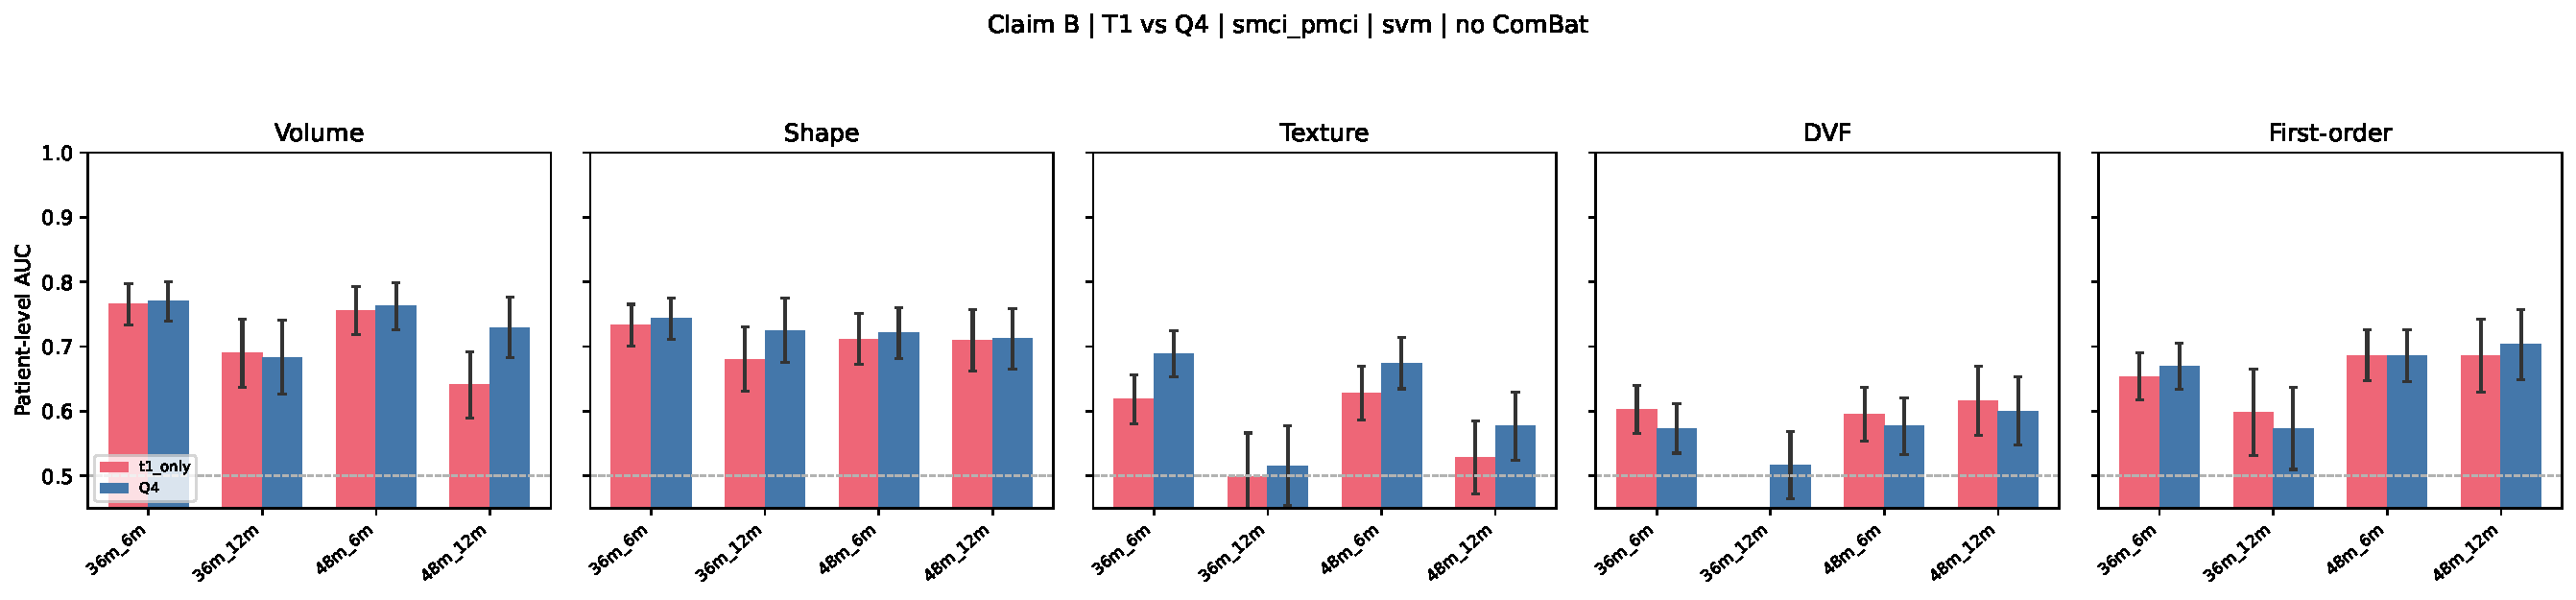
\includegraphics[width=\linewidth]{figures/cohort_encoding_vs_t1_modalities.pdf}
	\caption{AUC no paciente por família, coorte e representação (\code{wide}, \code{t1\_only}, \code{t1\_deltas}).
		SVM, sem ComBat, sMCI$\times$pMCI.
		Barras de erro: SD bootstrap da AUC paciente.
		\code{wide} é âncora de níveis, não o contraste temporal (verde vs vermelho).}
	\label{fig:encoding}
\end{figure}

Sanidade CN$\times$AD: o mesmo stack em volume \code{t1\_deltas} em \code{48m\_12m} atinge AUC paciente $0.837$.
Valida extração e CV quando a separação anatómica é grande; o endpoint permanece sMCI/pMCI.
Não se usa ROC de volume \code{wide} nem heatmap modalidade$\times$classificador no corpo --- são a âncora A (história volume-\code{abs}).

% -----------------------------------------------------------------------------
\subsection{Fusão âncora}

O teto de forma no $t_0$ é $0.761\pm0.043$.
Uniões tardias só com \code{t1\_only} ficam perto desse teto.
A âncora pré-especificada forma@$t_0$ $\cup$ textura-$\Delta$ atinge $0.801\pm0.040$ (Tabela~\ref{tab:early_late}).
Tardia $>$ precoce na mesma especificação ($+0.029$): a concatenação dilui a forma; a média de scores preserva o braço de textura-$\Delta$.
Elastic-net e ComBat \textbf{não} substituem este endpoint (no v2, ``melhor imagem'' $=0.708$ vol+EN+ComBat era outro protocolo).

% -----------------------------------------------------------------------------
\subsection{Preditores clínicos e fusão}

Em \code{48m\_12m}, o SVM clínico de $t_0$ (sexo, idade, MMSE, ADAS, FAQ) atinge AUC paciente $0.812$ (permutação $p=0.0002$).
Forma \code{wide}: $0.783$.
Fusão precoce clínica$+$forma em \code{t1\_only}: $0.853$.
A L1 aplica-se só às colunas de imagem; o clínico entra $z$-scoreado no treino.

Bootstrap pareado: imagem \code{wide} vs clínico, $\Delta=-0.029$, IC95\% $[-0.132,0.075]$, $p$ bilateral $0.57$.
Fusão vs clínico: $\Delta=+0.041$, $[-0.016,0.100]$, $p=0.15$ (NS).
Fusão vs imagem: $\Delta=+0.070$, $[0.015,0.129]$, $p=0.016$, $q_{\mathrm{FDR}}=0.025$.
A RM hipocampal é adjunto: sozinha não bate os escores; acrescentá-la não fecha ganho robusto neste $n$.

% -----------------------------------------------------------------------------
\subsection{Atalho demográfico}

Em \code{36m\_6m}, idade só: AUC $0.560$ (permutação $p=0.057$); sexo só: $0.452$ ($p=0.901$).
Volume \code{wide}: $0.761$ ($p=0.0002$).
$\Delta$ imagem $-$ idade $=+0.201$, IC95\% $[0.119,0.282]$; imagem $-$ sexo $=+0.309$, $[0.200,0.417]$.
(Os $0.456$/$0.507$ do v2 eram a coorte legado $n=243$.)

% -----------------------------------------------------------------------------
\subsection{Sensibilidade: ComBat}

Em \code{36m\_6m}, representação \code{wide},
$\Delta=\mathrm{AUC}(\mathrm{sem\,ComBat})-\mathrm{AUC}(\mathrm{ComBat})$:
volume $+0.016$ (NS); forma $+0.018$ (NS); textura $-0.029$ (ComBat \emph{ajuda} pontualmente); deslocamento $+0.026$ ($q=0.049$).
Efeito inconsistente; o primary permanece sem ComBat.
Não se afirma que a variância entre centros seja menor que o sinal biológico.
Não se reproduz a fig.\ \code{combat.pdf} do v2 (volume $0.680\to0.700$ na coorte antiga).
	% =============================================================================
	\section{Discussão}
	\label{sec:discussao}
	
	A pergunta era se há alteração hipocampal útil no tempo para sMCI versus pMCI.
	A resposta é família-específica e estatisticamente modesta.
	
	\paragraph{Alteração não é concatenação.}
	\code{wide} empilha níveis de três visitas e pode subir a AUC sem isolar mudança.
	O contraste que responde à pergunta é \code{t1\_deltas} versus \code{t1\_only}.
	Além disso, a seleção por grupo opera sobre as colunas disponíveis em cada representação: o $\Delta$AUC compara pipelines completos, não o efeito causal isolado de acrescentar $t_1$ e $t_2$ sob as mesmas colunas~\cite{meinshausen-2010}.
	
	\paragraph{Forma teto, textura muda.}
	A geometria já discrimina no $t_0$; acrescentar deltas de forma não ajuda e por vezes piora.
	A textura GLCM é o único bloco com $\Delta>0$ nas quatro células do fatorial.
	O máximo ($+0.058$) coincide com a janela longa e o intervalo de 12 meses, mas o IC cruza zero e o FDR não fecha.
	Trata-se de um padrão direcional a confirmar, não de uma reivindicação de superioridade.
	
	\paragraph{Fatorial, não crowning.}
	As quatro coortes testam se o padrão sobrevive a janela e intervalo.
	Não são quatro réplicas: as populações sobrepõem-se e a janela muda quem entra.
	\code{48m\_12m} tem $n=120$ e 69\% dos pMCI com $i_3$ já em AD; é a célula mais frágil para um claim único, ainda que seja onde o $\Delta$ de textura é maior.
	
	\paragraph{Fusão tardia.}
	A âncora forma@$t_0$ $\cup$ textura-$\Delta$ segue a leitura unimodal: conservar o teto estático e acrescentar o único bloco que se move.
	Late $>$ early na mesma especificação ($+0.029$) alinha-se com diluição da forma na seleção conjunta.
	
	\paragraph{Clínico primeiro.}
	AUC clínica $0.81$ versus forma de imagem $\approx 0.76$--$0.78$ reproduz o recado da literatura~\cite{grassi-2019,moradi-2015}: na ADNI, escores de $t_0$ já carregam muito do prognóstico.
	A arquitetura de apoio à decisão é palco: clínico barato na frente; RM só onde demonstrar valor incremental sob a mesma validação.
	O ganho fusão versus clínico não foi significativo neste $n$.
	
	\paragraph{Deslocamento.}
	O DVF v2 mede desvio ao template CN, não warp entre visitas.
	AUC perto do acaso em \code{48m\_12m} é coerente com ROI pequena, interpolação SyN e ausência de deformação inter-visita explícita.
	Publicar esse negativo evita otimismo em descritores caros sob validação estrita~\cite{cuingnet-2011}.
	
	% =============================================================================
	\section{Limitações}
	\label{sec:limitacao}
	
	\begin{itemize}
		\item \textbf{Uma fonte, caso completo.} Só a ADNI fornece $n$ viável com três RM e rótulo sMCI/pMCI nas janelas 36/48 meses.
		AIBL e OASIS foram rastreadas no mesmo fluxo; após a exigência de triplets restavam poucos sujeitos, sobretudo pMCI.
		Relaxar para uma ou duas visitas quebraria a comparabilidade com $t_0$+deltas.
		\item \textbf{Soft pMCI.} 46 pacientes em intervalos de 6 meses e 33 em intervalos de 12 meses têm $i_3$ igual ao primeiro AD.
		Parte do sinal longitudinal pode ser atrofia já pós-conversão.
		\item \textbf{Sobreposição e $n$.} Coortes não independentes; \code{48m\_12m} tem 120 sujeitos para nested CV, seleção e fusão.
		\item \textbf{Operações pré-CV.} Limites de QC e templates CN estimam-se uma vez no conjunto, não dentro de cada dobra.
		Os templates não contêm sMCI/pMCI.
		\item \textbf{ROI única.} Hipocampo de propósito; subestima córtex entorrinal, lobo temporal ou cérebro inteiro.
		\item \textbf{Intensidade e radiómica.} Não houve ablação de histogram matching (não usado) nem de \code{binCount}.
		ComBat no nível do atributo não substitui ablação da cadeia de intensidade.
		\item \textbf{Seleção específica da representação.} O $\Delta$AUC não isola o contributo causal das visitas de seguimento.
	\end{itemize}
	
	% =============================================================================
	\section{Conclusões}
	\label{sec:conclusoes}
	
	Sob validação aninhada no paciente, a representação $t_0$+deltas não supera de forma estatisticamente robusta (FDR) o baseline unimodal em nenhuma das quatro famílias.
	Ainda assim o padrão é interpretável: a forma já discrimina no $t_0$; a textura é o único bloco com ganho de deltas nas quatro coortes; o volume é misto; o deslocamento normativo não contribui.
	A fusão tardia que junta o teto de forma ao braço de textura-$\Delta$ atinge AUC $0.80$ em \code{48m\_12m} e supera a fusão precoce na mesma especificação.
	Escores clínicos de $t_0$ permanecem o sinal de primeira linha; a RM hipocampal entra como adjunto estrutural.
	O contributo deste trabalho é o protocolo auditável --- elegibilidade temporal, fronteira de vazamento, fatorial janela$\times$intervalo e ablações negativas --- mais do que um classificador novo.
	
	% =============================================================================

\section{Discussão}
\label{sec:discussao}

Este estudo especifica e estressa um pipeline longitudinal de atributos hipocampais na ADNI, com sMCI versus pMCI como desfecho.
A interpretação está ligada ao fatorial de elegibilidade: quatro células (janelas 36/48\,meses $\times$ intervalos nominais 6/12\,meses, tolerância $\pm 2$), três preditoras por sujeito, desfecho na mesma janela clínica, e $i_3=$ primeiro AD só quando faltam três MCI (46 nos intervalos de 6 meses; 33 nos de 12).
Não é o protocolo legado de uma só janela de 36 meses com gap $\ge 6$ e $n=243$.
A avaliação usa CV aninhada no paciente, AUC OOF agregada por sujeito, permutação contra o acaso e bootstrap pareado.
Operações sample-dependent ajustam-se dentro da validação; pré-processamento por imagem, QC de conjunto e templates CN ocorrem antes da CV.
Essa fronteira importa: o desempenho infla quando informação de conversão, selecção, harmonização ou limiar usa o que não estaria disponível no instante da previsão.
A contribuição não é mais um classificador isolado, e sim uma arquitectura de avaliação em que hipóteses temporais, fronteiras de ajuste, estimandos e ablações negativas são inspectáveis --- reutilizável para componentes de apoio à decisão em neuroimagem, onde um modelo «mais forte» só conta se o ganho sobrevive aos mesmos controlos de vazamento.

\subsection{Desempenho prognóstico e dificuldade da tarefa}

A pergunta era se há alteração hipocampal útil no tempo além do $t_0$.
A resposta é família-específica e estatisticamente modesta: nenhum $\Delta$AUC unimodal retém $q<0.05$ após FDR-BH nas quatro modalidades de cada coorte.

A forma é um teto estático: em \code{48m\_12m}, \code{t1\_only} $0.761\pm0.043$ e os deltas não superam o baseline ($0.736$).
A textura GLCM é o único bloco com $\Delta>0$ nas quatro células (máximo $+0.058$ em \code{48m\_12m}, $p=0.053$, $q=0.212$): padrão direccional, IC a cruzar zero, não reivindicação de superioridade.
Volume é misto; deslocamento é fraco ou negativo (em \code{36m\_12m} o IC do $\Delta$ favorece $t_0$).
Hierarquia prática dos tetos unimodais: forma $\gg$ textura $\gtrsim$ volume $\gg$ deslocamento.
Isto inverte o ranking do rascunho v2 (volume $\gg$ forma $\gg$ textura/deslocamento em representação \code{wide}).

AUC de imagem $\approx 0.76$ no teto de forma está acima do acaso e ainda aquém do limiar frequentemente citado para estratificação individual ($\mathrm{AUC}\gtrsim 0.80$), salvo a fusão tardia âncora ($0.801\pm0.040$), que mesmo assim não supera o clínico de $t_0$ ($0.812$).
Idade e sexo não explicam o sinal: em \code{36m\_6m}, idade só $0.560$, sexo só $0.452$; volume \code{wide} retém $\Delta$ vs idade $+0.201$ e vs sexo $+0.309$.
O sinal é hipocampal, não proxy demográfico; a magnitude absoluta permanece modesta, coerente com ROI única e conversão heterogénea~\cite{wyman-2013,scheltens-1992,cuingnet-2011}.

\code{wide} vs \code{t1\_only} não é o contraste que responde à pergunta temporal: concatenar níveis pode subir a AUC sem isolar mudança.
O contraste oficial é \code{t1\_deltas} vs \code{t1\_only}.
Além disso, o pool L1 opera sobre as colunas de cada representação: o $\Delta$AUC compara pipelines completos, não o efeito causal de acrescentar $t_1$ e $t_2$ sob as mesmas colunas~\cite{meinshausen-2010}.

\subsection{Ablações por família}

Publicar textura e deslocamento não é preenchimento: sob nested fold-wise, documentam o que sobrevive e o que não.
A textura \textbf{não} está no acaso neste protocolo (p.ex.\ $0.753$ em deltas, \code{48m\_12m}); o que falha ao FDR é o \emph{ganho} dos deltas, não a discriminação absoluta.
O deslocamento normativo (desvio ao template CN, não warp $T_a\to T_b$) fica perto do acaso em \code{48m\_12m}, coerente com ROI pequena, interpolação SyN e ausência de deformação inter-visita explícita.

Mecanismos, não mutuamente exclusivos:
(i)~ROI compacta: diferenças subtis; SyN e reamostragem ampliam erro de interpolação, que pune DVF e textura local;
(ii)~ADNI mistura 1.5\,T e 3\,T; descritores de intensidade são os mais sensíveis, e o primary não usa ComBat --- de facto a textura \emph{melhora} pontualmente com ComBat em \code{36m\_6m} \code{wide};
(iii)~mesmo com allowlist compacta e L1, o efeito biológico sMCI/pMCI é pequeno face à variância;
(iv)~fracções teciduais e forma ligam-se directamente à atrofia clássica~\cite{wyman-2013}; o espaço fundido cedo dilui o teto de forma.

Estudos com textura mais forte podem ter beneficiado de pré-processamento global, selecção no teste ou splitting menos conservador.
O benchmark negativo do DVF desencoraja vazamento analítico em descritores caros.

\subsection{Imagem versus clínico e fusão}

Escores de $t_0$ (sexo, idade, MMSE, ADAS, FAQ) superam a imagem hipocampal isolada: clínico $0.812$ vs forma \code{wide} $0.783$ em \code{48m\_12m}.
A fusão precoce clínica$+$forma em \code{t1\_only} chega a $0.853$, mas vs clínico $\Delta=+0.041$, IC $[-0.016,0.100]$, $p=0.15$ (NS).
Fusão vs imagem: $\Delta=+0.070$, $q=0.025$.
A RM sozinha não bate o clínico; acrescentá-la não fecha ganho robusto neste $n$.
Isso reproduz o recado de~\citet{grassi-2019,moradi-2015}: na ADNI, cognição de baseline já carrega muito do prognóstico.

Não implica que a RM seja irrelevante em geral.
Pode exigir outras ROIs (entorrinal, lobo temporal), modelos de progressão explícitos, coortes multi-sítio maiores, ou fusão só em casos clinicamente ambíguos --- análise em aberto.
A fusão tardia imagem-imagem (forma@$t_0$ $\cup$ textura-$\Delta$, média de scores) \textbf{foi} avaliada e supera a precoce na mesma especificação ($+0.029$): a selecção conjunta dilui a forma; a média de scores preserva o braço de textura-$\Delta$.
Isso não substitui o clínico.

\subsection{Implicações para apoio à decisão}

A evidência favorece arquitectura em palco, não preditor com RM primeiro.
Variáveis clínicas baratas na frente; atributos de RM só onde demonstrarem valor incremental num subgrupo ou decisão pré-definidos.
O pipeline actual é a camada de validação: testa se representação longitudinal, família, ComBat ou fusão acrescentam discriminação no paciente depois de isolar do teste tudo o que é treinável.
Os resultados \textbf{não} justificam implantação nem substituição da avaliação clínica.
Avaliação prospectiva, calibração em pontos operacionais, validação externa e benefício clínico líquido continuam necessários.

\section{Limitações}
\label{sec:limitacao}

\begin{itemize}
	\item \textbf{Uma fonte, caso completo.} Só a ADNI fornece $n$ viável com três RM e rótulo sMCI/pMCI nas janelas 36/48 meses.
	AIBL e OASIS foram rastreadas; após triplets restavam poucos sujeitos, sobretudo pMCI.
	\item \textbf{Soft pMCI.} 46 (intervalos de 6 meses) e 33 (12 meses) têm $i_3$ igual ao primeiro AD; parte do sinal longitudinal pode ser atrofia já pós-conversão.
	\item \textbf{Sobreposição e $n$.} Coortes não independentes; \code{48m\_12m} tem 120 sujeitos para nested CV, selecção e fusão.
	\item \textbf{Operações pré-CV.} QC do MRQy e templates CN estimam-se uma vez no conjunto.
	Os templates não contêm sMCI/pMCI.
	Não é um pipeline em que \emph{todas} as operações cabem nas dobras.
	\item \textbf{ROI única.} Hipocampo de propósito; subestima entorrinal, lobo temporal ou cérebro inteiro.
	\item \textbf{Intensidade e radiómica.} Não houve histogram matching neste repositório nem ablação de \code{binCount}.
	ComBat no atributo não substitui ablação da cadeia de intensidade.
	\item \textbf{Pré-processamento interno ANTsPyNet.} Parcelamento e deep Atropos com \code{do\_preprocessing=True} após cadeia ANTsX externa podem duplicar normalização face ao domínio dos pesos pré-treinados.
	\item \textbf{Selecção específica da representação.} O $\Delta$AUC não isola o contributo causal das visitas de seguimento.
	\item \textbf{Custo.} SyN, templates groupwise e radiómica limitam iteração rápida.
\end{itemize}

\section{Conclusões}
\label{sec:conclusoes}

Apresentámos um quadro longitudinal de atributos hipocampais e classificação prognóstica na ADNI (ADNI-1/2/GO), avaliado com CV aninhada no paciente.
Quatro coortes (36/48\,meses $\times$ 6/12\,meses, $\pm 2$); inclusão ampliada MCI--MCI--AD quando necessário.
A contribuição principal é o protocolo auditável --- elegibilidade temporal, fronteira de vazamento, fatorial, ablações e inferência no paciente --- não um classificador novo.

Sob esse protocolo, $t_0$+deltas \textbf{não} supera de forma estatisticamente robusta (FDR) o baseline unimodal em nenhuma das quatro famílias.
O padrão é interpretável: a forma já discrimina no $t_0$; a textura é o único bloco com ganho de deltas nas quatro coortes; o volume é misto; o deslocamento normativo não contribui.
A fusão tardia forma@$t_0$ $\cup$ textura-$\Delta$ atinge AUC $0.80$ em \code{48m\_12m} e supera a fusão precoce na mesma especificação.
Escores clínicos de $t_0$ permanecem o sinal de primeira linha ($0.81$ vs imagem $\approx 0.76$--$0.78$); a RM hipocampal entra como adjunto estrutural, e o ganho da fusão clínica$+$imagem versus clínico não foi significativo neste $n$.

A evidência sustenta arquitectura conservadora: clínico primeiro; RM estrutural só depois de demonstrar valor incremental sob a mesma validação.
Trabalho futuro: coortes externas, cobertura além do hipocampo, regras calibradas por subgrupo, e utilidade clínica sem quebrar o isolamento fold-wise de cada operação sample-dependent.

	\section*{Agradecimentos}
	
	A recolha e a partilha dos dados foram financiadas pela Alzheimer's Disease Neuroimaging Initiative (ADNI).
	
	\subsection*{Financiamento}
	
	O presente trabalho foi realizado com apoio da Coordenação de Aperfeiçoamento de Pessoal de Nível Superior -- Brasil (CAPES) -- Código de Financiamento 001.
	
	\section*{Conflito de interesses}
	
	Os autores declaram não haver conflito de interesses.
	
	\bibliographystyle{cas-model2-names-short}
	\biboptions{authoryear}
	\bibliography{referencias}
\end{document}
